\documentclass[twocolumn,english,notitlepage]{article}
\usepackage[margin=0.5in]{geometry}
% \setlength{\parindent}{0pt} % no indents

% Math
\usepackage{amsmath}
\usepackage{physics}
\usepackage{amsfonts} % for mathbb

% Citetations
\usepackage[ backend=bibtex, sorting=none, autocite=plain]{biblatex}
\addbibresource{refs/references}
\usepackage{xcolor}
\usepackage{hyperref}
\hypersetup{
    colorlinks,
    linkcolor={red!50!black},
    citecolor={blue!50!black},
    urlcolor={blue!80!black}}


% Formatting
\usepackage{float}
\usepackage{graphicx}
\usepackage{subcaption}

\graphicspath{ {./figs/} } 

% Misc
\usepackage{appendix}
\usepackage{xfrac} % provides \sfrac

% Commands

\newcommand{\comment}[1]{\textcolor{red}{#1}}

\newcommand{\integral}[1]{\ensuremath{\int\!\mathrm{d}#1\,}}
\renewcommand{\d}[2][x]{\ensuremath{\frac{\mathrm{d}#2}{\mathrm{d}#1}}}

\renewcommand{\vec}[1]{\boldsymbol{#1}}
\newcommand{\pclosed}[1]{\left(#1\right)}
\newcommand{\bclosed}[1]{\left[#1\right]}
\newcommand{\cclosed}[1]{\left\{#1\right\}}
\newcommand{\vclosed}[1]{\left|#1\right|}
\renewcommand{\norm}[2][]{\ensuremath{\|#2\|_{#1}}}
\renewcommand{\exp}[1]{e^{#1}}
\newcommand{\exptext}[1]{\operatorname{exp}\pclosed{#1}}
\newcommand{\dimof}[1]{\bigl[#1\bigr]}
\newcommand{\normal}[2]{\operatorname{\mathcal{N}}\pclosed{#1,#2}}

\newcommand{\distas}{\overset{d}{\sim}}
\renewcommand{\expval}{\operatorname{\mathbb{E}}}
\DeclareMathOperator{\mse}{MSE}
\renewcommand{\var}{\operatorname{Var}}
\newcommand{\bias}{\operatorname{Bias}}
\DeclareMathOperator{\Rsquared}{R^2}
\DeclareMathOperator{\eye}{\mathbb{I}}
\DeclareMathOperator{\sgn}{sgn}

\newcommand{\thetahat}{\hat{\theta}}
\newcommand{\msub}[2]{\ensuremath{{#1}_\text{#2}}}

\newcommand{\Hakon}{$\mathcal{H}$}
\newcommand{\Carl}{$\mathbb{CM}$}
\newcommand{\Anna}{$\mathfrak{Anna}$}

\title{Bias-Variance Tradeoff in Simple Linear Models}
\author{Anna Aasen, Carl Martin Fevang, Håkon Kvernmoen}
\date{\today}

\begin{document}

\twocolumn[
    \begin{@twocolumnfalse}
        \maketitle
        \begin{abstract}
            This is the abstract.
        \end{abstract}
    \end{@twocolumnfalse}
]

\section{Introduction}
    In this project, we will introduce some of the most important general properties of machine learning models in the context of linear regression. Specifically the mean squared error (MSE), the bias, and the variance of data predictions are essential in evaluating the quality of a statistical model. We look at the phenomena of underfitting and overfitting, and explore them in the context of bias-variance trade-off. The three models we will use explicitly are Ordinary Least Squares (OLS), Ridge regression and Least-Absolute-Shrinkage-and-Selection-Operation (Lasso) regression. These will first be tested on the 2D Franke function, and later on real geographical terrain data.

    The aforementioned models will be explored using resampling techniques, which will be employed to extract the relevant statistical quantities in an accurate way. We will use the standard methods of Bootstrapping and $k$-fold Cross Validation and compare the results we get between them across the three linear models.

    All the models will be applied by fitting a two-dimensional polynomial expansion to the observed data.

\section{Theory}
    Before we delve into to details of the theory section, it is useful to take a moment to define the quantities we will be dealing with. Let $\vec{y}$ denote a vector of a series of measured values $y_i$, $i\in 1, 2,\ldots, n$ at points $X$, where $X$ is a matrix where the rows $x_i$ correspond to the input values that produced the measurement $y_i$. For completeness we refer to the columns of $X$ as $\vec{x}_a$, $a=1, 2,\ldots, p$.\footnote{Throughout this project, $a, b$ will always index the $p$ features for a model, and $i, j$ the $n$ data points.} Together, these form the dataset $\mathcal{D} = \cclosed{(y_i, x_i)}$. Another important set of values is $\vec{\theta}$ which contains the parameters that will define the model we will use to predict the data.

    We will assume that the measurements $y_i$ are generated from an exact function $f(x)$ with stochastic noise $\epsilon$ added, such that $y_i = f(x_i) + \epsilon$. Throughout this project, we will assume that the noise is normally distributed with zero mean and some standard deviation (std) $\sigma$; $\epsilon \distas \normal{0}{\sigma^2}$. Furthermore, we will assume that the noise between different measurements is independent and identically distributed (i.i.d.). Our job then is to model an $\hat{f}(x)$ that we want to be close to $f(x)$.

    \subsection{Error assessment and model optimisation}

    \subsubsection*{Measure for goodness of fit}
        When we want to create a statistically informed model that is able to predict the outcome of future measurements, we need to develop metrics for how well our model fits the data we already have. That is, given a model parametrised by parametrs $\vec{\theta}$, we want to optimise them such that $\hat{f}(x) \approx f(x)$. We call this the goodness of fit. To estimate how well we acheive this with our given dataset $\mathcal{D}$, we will start with the mean squared error (MSE). Given a model which predicts values $\vec{\hat{y}}$, the mean squared error is given by
        \begin{align}
            \mse(\vec{\hat{y}}) = \frac{1}{n} \sum_{i=1}^n (y_i-\hat{y}_i)^2 = \frac{1}{n} (\vec{y} - \vec{\hat{y}})^2,
            \label{theo:eq:mse}
        \end{align}
        and is a strictly positive metric that we want to minimise.

        Another popular metric we will use to evaluate the goodness of fit is the $\Rsquared$-score, calculated as
        \begin{align}
            \Rsquared(\vec{\hat{y}}) = 1 - \frac{\sum_{i=1}^n (y_i-\hat{y}_i)^2}{\sum_{i=1}^n (y_i-\bar{y})^2} = 1 - \frac{(\vec{y}-\vec{\hat{y}})^2}{(\vec{y}-\bar{y})^2},
            \label{theo:eq:r2}
        \end{align}
        where $\bar{y} = \frac{1}{n}\sum_{i=1}^n y_i$ is the sample mean of the observed data. This metric falls on the interval $(-\infty, 1]$, where 1 denotes the perfect fit, 0 correspond to a constant prediction of $\hat{y}_i = \bar{y}$, and negative values corresponds to worse prediction than this.


        To get further insight into the validity of our model, we can decompose the MSE into its \textit{bias} and \textit{variance}, which are quantities that can tell us more about exactly what our model is doing wrong. To set up this decomposition, we consider a situation where we have fitted a model to a series of $L$ different datasets, with parameters $\vec{\hat{\theta}}^\ell$, with $\ell=1,\ldots,L$, and predictions $\vec{\hat{y}}^\ell$ on the dataset we want to compare to. The sample mean squared error at each observed point can then be decomposed into
        \begin{align}
            \mse(\hat{y}_i) = \pclosed{\bias(\hat{y}_i)}^2 + \var(\hat{y}_i),
        \end{align}
        where 
        \begin{subequations}
            \begin{align}
                \bias(\hat{y}_i) &= \frac{1}{L}\sum_{\ell=1}^L \pclosed{y_i - \hat{y}_i^\ell}, \\
                \var(\hat{y}_i) &= \frac{1}{L}\sum_{\ell=1}^L \pclosed{\hat{y}_i^\ell - \frac{1}{L} \sum_{m=1}^L \hat{y}_i^m }^2,
            \end{align}
            \label{theo:eq:bias and var}
        \end{subequations}
        are the sample bias and sample variance of the model at the predicted point. This decomposition is done in more detail in Appendix~\ref{app:sec:bvdecomp}. 


    \subsubsection*{Central Limit Theorem}
        The central limit theorem tells us that when sampling a series of quantities $\cclosed{z_i|i=1,\ldots,n}$ with independent and identical distributions with a mean $\mu$ and variance $\sigma^2<\infty$, the distribution of the sample mean $\bar{z}_n = \frac{1}{n}\sum_{i=1}^n z_i$ will approach a normal distrbution. Explicitly, we have
        \begin{align}\label{theo:eq:CLM}
            \lim_{n\to\infty} \sqrt{n}(\bar{z}_n-\mu) \distas \normal{0}{\sigma^2}.
        \end{align}
        In practice, for some notion of a large sample size $n$, the approximation of the sample mean as being distributed as
        \begin{align}
            \bar{z}_n \distas \normal{\mu}{\frac{\sigma^2}{n}}
        \end{align}
        becomes sound. Colloquially we say the sample mean approaches the true mean $\mu$. This is powerful, as it means not only that the sample mean becomes better as the sample size grows, but quantities derived from its distribution are also determined more precisely. Note also that this holds with only very weak restrictions on the distribution of the $z_i$'s -- their sample mean will approach normal distribution regardles. This lays the foundation for statistically informed models such as regression methods.

        


    \subsection{Statistical introduction to linear regression}
        A way to motivate the process of statistical learning is that we want to develop a process by which we use observed data to inform our belief in a future outcome. Such a process can be developed from the ideas of Bayes' theorem, which we can use to inform us what confidence we should have in the parameters of a given model, given data points we have observed.
        
        Bayes' theorem tells us that our \textit{posteriori} confidence in the parameters $\vec{\theta}$, given the available dataset $\mathcal{D}=(\vec{y}, X)$, is given by the probability
        \begin{align}
            P(\vec{\theta}|X, \vec{y}) = \frac{P(\vec{y}|X,\vec{\vec{\theta}})P(\vec{\theta})}{P(X,\vec{y})},
        \end{align}
        where $P(\vec{y}|X, \vec{\theta})$ is the \textit{likelihood} of observing the values $\vec{y}$ at points $X$ given parameters $\vec{\theta}$, and $P(\vec{\theta})$ is our \textit{prior} confidence in $\vec{\theta}$, before the data was seen. $P(X,\vec{y})$ plays the role of a normalisation, and can safely be ignored -- either because we look for values of $\vec{\theta}$ that maximise the probability, or because we assume the probabilities $P(\vec{y}|X,\vec{\theta})$ and $P(\vec{\theta})$ which we can then properly normalise. Now we have a framework through which we can build a model by making assumptions about the probability distributions $P(\vec{y}|X,\vec{\theta})$ and $P(\vec{\theta})$ to give us a probability distribution for the parameters $\vec{\theta}$ that we can maximise.


        \subsubsection{Ordinary least squares}
            We define the ordinary least squares method by assuming that the data $y(x)$ that we want to make a fit to has a linear noise term that is normally distributed with zero mean. That is, the data is generated as $y(x) = f(x) + \epsilon$, where $f(x)$ is some analytic, non-stochastic function of the data input $x$, and $\epsilon \distas \normal{0}{\sigma^2}$ for some $\sigma^2>0$. Further, if we make a model fitting $y(x)$ by a $\hat{y}(x)$, we should expect the error at every data point $(y_i, x_i)$ to be be normally distributed with the same variance, i.e., independently and identically distributed (i.i.d.). This can be summarised
            \begin{align}
                P(\vec{y}|X, \vec{\theta}) = \prod_{i=1}^{n} \frac{1}{\sqrt{2\pi\sigma^2}} \exp{-\frac{{(y_i-\hat{y}_i)}^2}{2\sigma^2}}.
            \end{align}
            Furthermore, we assume the parameters $\vec{\theta}$ to be distributed uniformly, and as such, $P(\vec{\theta})$ just contributes to an overall normalisation. This means that maximising $P(\vec{y}|X, \vec{\theta})$ amounts to the same as maximising $P(\vec{\theta}|X, \vec{y})$, and can be done analytically.

            Knowing that the Gaussian distribution has a single extremum that is a maximum, we can find the values for $\vec{\theta}$ maximising the probability from
            \begin{align} \nonumber
                \d[\theta_k]{P(\vec{y}|X,\vec{\theta})} &= 0 \\
                \Rightarrow \prod_{i=1}^{n} \frac{1}{\sqrt{2\pi\sigma^2}} \frac{1}{\sigma^2} X_{ib}(y_i-X_{ia}\theta_a) \exp{-\frac{{(y_i - X_{ia}\theta_a)}^2}{2\sigma^2}} &= 0,
            \end{align}
            which as we can see, is maximisable point by point. This means that the optimal parameters $\msub{\vec{\hat{\theta}}}{OLS}$ that maximise $P(\vec{y}|X, \vec{\theta})$ are given analytically by
            \begin{align}
                \boxed{
                    \msub{\vec{\hat{\theta}}}{OLS} = \pclosed{X^TX}^{-1} X^T \vec{y}.
                    \label{theo:eq:OLS_coefs}
                }
            \end{align}
            An exploration of the statistical expectation and variance of the OLS results is done in Appendix~\ref{app:sec:OLS_proof}.

        \subsubsection{Ridge regression}
            So far, we have assumed that the parameters $\vec{\theta}$ are uniformly distributed, and as such have no \textit{bias} towards any particular value. In practice, this means that the OLS model will contort to fit itself to all values in the data. As such, a motivation for adding a bias could be for the sake of stability in the fit. These methods are called \textit{regularised} methods. An example is ridge regression, where one assumes that the parameters are normally distributed, such that parameter values far from the mean are thought less likely to occur. This in practice means that the model is less willing to contort to outliers in the dataset, trading it for a bias towards certain parameter values. Assuming the probability distrbution for $\theta_a \distas \normal{0}{\tau^2}$,
            \begin{align}
                P(\vec{\theta}) = \prod_{a=1}^{p} \frac{1}{\sqrt{2\pi\tau^2}} \exp{-\frac{\theta_a^2}{2\tau^2}},
            \end{align}
            with a derivative with respect to $\theta_b$
            \begin{align}
                \d[\theta_b]{P(\vec{\theta})} = -\prod_{a=1}^{p} \frac{1}{\sqrt{2\pi\tau^2}} \frac{1}{\tau^2} \theta_b \exp{-\frac{\theta_a^2}{2\tau^2}} = -\frac{1}{\tau^2} \theta_b P(\vec{\theta}),
            \end{align}
            the condition for maximising $P(\vec{\theta}|X, \vec{y})$ becomes
            \begin{align} \nonumber
                \d[\vec{\theta}]{P(\vec{y}|X, \vec{\theta})} P(\vec{\theta}) + P(\vec{y}|X, \vec{\theta}) \d[\vec{\theta}]{P(\vec{\theta})} &= 0 \\
                \pclosed{ \frac{1}{\sigma^2} X^T(\vec{y}-X\vec{\theta}) - \frac{1}{\tau^2} \vec{\theta} } P(\vec{y}|X,\vec{\theta}) P(\vec{\theta}) &= 0.
            \end{align}
            Rewriting with a parameter $\lambda = \sigma^2/\tau^2$, the optimal parameters $\msub{\vec{\hat{\theta}}}{ridge}$ are given by
            \begin{align}
                \boxed{
                \msub{\vec{\hat{\theta}}}{ridge} = \pclosed{X^TX + \lambda \eye}^{-1} X^T \vec{y}.
                \label{theo:eq:Ridge_coefs}
                }
            \end{align}
            This has the added bonus of ensuring that $X^TX + \lambda \eye$ is always invertible, as $\det(\lambda \eye) \neq 0$ for $\lambda>0$.


        \subsubsection{Lasso regression}
            Lasso regression builds on the same ideas as ridge regression, but rather assumes parameters $\vec{\theta}$ are distributed according to the Laplace distribution $L(0, \tau)$. This looks like
            \begin{align}
                P(\vec{\theta}) = \prod_{a=1}^{p} \frac{1}{2\tau} \exp{-\frac{|\theta_a|}{\tau}},
            \end{align}
            which as we can see is not differentiable at $\theta_a = 0$. This means that the optimisation of the probability $P(\vec{\theta}|X, \vec{y})$ is not necessarily possible analytically without putting bounds on the data $X, \vec{y}$, and even numerical algorithms like gradient descent will encounter trouble. Moreover, it is not optimisable point by point, unless bounds like $X^TX$ being diagonal are enforced. This makes Lasso generally more cumbersome. Nevertheless, we can coax a cost function out of the probability, which is minimalisable. Letting the cost function be written $\msub{C}{lasso}(\vec{\theta}) = -A\log\pclosed{P(\vec{\theta}|X,\vec{y}}) + B$  we can choose the constants $A, B$ such that
            \begin{align}
                \boxed{
                    \msub{C}{lasso}(\vec{\vec{\theta}}) = \norm[2]{ \vec{y} - X\vec{\theta} }^2 + \lambda \norm[1]{\vec{\theta}},
                }
                \label{theo:eq:Lasso_costfunction}
            \end{align}
            where $\lambda = \frac{2\sigma^2}{\tau}$ and $\norm[p]{\vec{v}} = \pclosed{\sum_k |v_k|^p}^{\sfrac{1}{p}}$ denotes the $L_p$ norm of the vector $\vec{v} \in \mathbb{R}^k$.


\section{Method}
    Something general about initially fitting Franke data using OLS, ridge and Lasso. Then moving on to real terrain data something something.
    
    \subsection{Datasets}
        \subsubsection*{Franke function}

            For the initial testing of our implemented fitting routines, we will use the so called \textit{Franke function}. Being able to control the number of sample points and noise levels will serve as a good examination of our models advantages and disadvantaged. Defined for $x, y \in [0,1]$

            \begin{align}
                F(x,y) = f_1(x,y) + f_2(x,y) + f_3(x,y) + f_4(x,y) + \epsilon \label{met:eq:Franke_Function}
            \end{align}

            Where the $f_i(x,y)$ are Gaussian functions, constructed to mimic the shape of a hill top landscape. More concretely, these are defined as:

            \begin{align} \nonumber
                f_1(x,y) &= \frac{3}{4}\exptext{ -\frac{(9x-2)^2}{4} - \frac{(9y-2)^2}{4} } \nonumber \\
                f_2(x,y) &= \frac{3}{4}\exptext{ -\frac{(9x+1)^2}{49} - \frac{(9y+1)}{10}} \nonumber \\
                f_3(x,y) &= \frac{1}{2}\exptext{ -\frac{(9x-7)^2}{4} - \frac{(9y-3)^2}{4}} \nonumber \\
                f_4(x,y) &= -\frac{1}{5}\exptext{ -(9x-4)^2 - (9y-7)^2} \nonumber
            \end{align}

            And $\epsilon$ is some stochastic noise $\epsilon \distas \normal{0}{\sigma^2}$. By visual inspection, we can fine tune $\sigma$ to create data that looks like noisy digital terrain data. Unless specified otherwise all fits to the Franke function will use $n = 600$ uniformly distributed points $x,y \distas \mathcal{U}(0,1)$ with a noise level of $\sigma = 0.1$. We discuss this in in Appendix~\ref{app:sec:frankefunction N and sigma}.   

        \subsubsection*{Terrain data}
            \comment{Here we put the terrain we extracted with coordinates etc.}\\
            We chose to sample terrain data from a mountainous region in northwestern Nicaragua, close to the border to Honduras, see Figure~\ref{met:fig:gmaps}.
            The terrain data consists of a 300 by 300 point grid with one arcsecond ('') resolution. When doing our fits, we restrict our data to $n=600$, as in the earlier case of the Franke function. The points are sampled uniformly from the grid, without replacement. 
            \begin{figure} [ht]
                \centering
                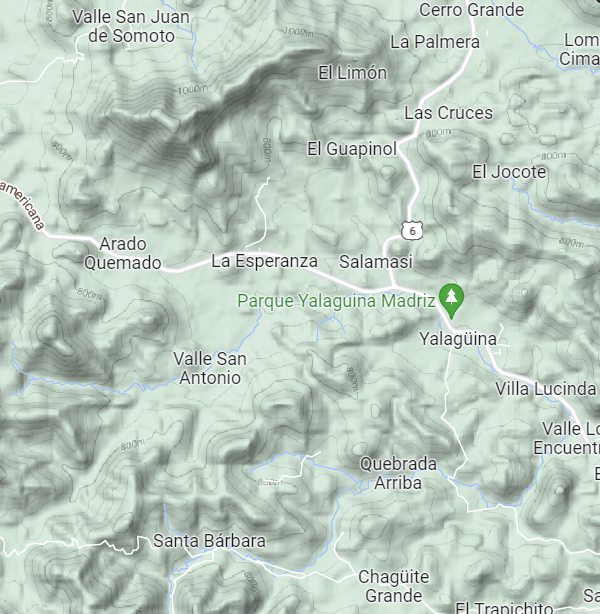
\includegraphics[width=.9\linewidth]{Nica_gmaps.PNG}
                \caption{Map of the terrain taken from \url{google.com/maps}. \\
                Coordinates of south-west corner: $13^\circ\,26'\,40''\,\text{N}, 86^\circ\,33'\,20''\,\text{W}$ \\
                Coordinates of north-east corner: $13^\circ\,31'\,40''\,\text{N}, 86^\circ\,28'\,20''\,\text{W}$}
                \label{met:fig:gmaps}
            \end{figure}
            

        \subsection{Data preparation}
            When fitting our models to the data, we base our models on simple polynomial expansions of the arguments of the function generating the data. We are fitting scalar function with two arguments $x$ and $y$, so our design matrix is constructed as
            \begin{align} \label{met:eq:design_X}
                X = \begin{pmatrix}
                    1 & x_1 & y_1 & x^2_1 & x_1y_1 & y_1^2 & \cdots & x_1^p & \cdots & y_1^p \\
                    \vdots & \vdots & \vdots & \vdots & \vdots & \vdots & \vdots & \vdots & \ddots & \vdots \\
                    1 & x_n & y_n & x^n_n & x_ny_n & y_n^2 & \cdots & x_n^p & \cdots & y_n^p
                \end{pmatrix}
            \end{align}
        
            Before fitting the models to the sampled data, we will scale the data using the $Z$-score normalisation. This scales the inputs $x_i$ and the targets $\vec{y}$ such that they have a mean value of $0$ with a standard deviation $1$. In effect, we rescale
            \begin{subequations}
                \begin{align}
                    \vec{y} &\to \frac{\vec{y}-\bar{y}}{\bar{\sigma}_{\vec{y}}}, \\
                    \vec{x}_a &\to \frac{\vec{x}_a - \bar{x}_a}{\bar{\sigma}_{\vec{x}_a}},
                \end{align}
            \end{subequations}
            where $\bar{z} = \frac{1}{n} \sum_{i=1}^n z_n$ denotes the sample mean of $\vec{z}$ and $\sigma_{\vec{z}}^2 = \frac{1}{n} \sum_{i=1}^n {(z_i-\bar{z})}^2$ denotes the sample std of $\vec{z}$. When we calculate MSE scores to compare between models and resampling techniques, we will use the scaled $\vec{y}$.

            To get a proper assessment of our model, we will split the dataset into a \textit{training set} and \textit{testing set}. The training set is used to fit the model, giving our coefficient estimates $\vec{\hat{\theta}}$. Using the fitted model and the training data, we can calculate metrics to quantify how good our model replicates this data. In the case that our model perfectly predicts the training data $\vec{y}$ based on $X$, the calculated metrics MSE and $\Rsquared$ (Eqs.~\ref{theo:eq:mse},~\ref{theo:eq:r2}) should be 0 and 1 respectively. However, using these scores to assess the goodness of our fit has an underlying problem. Since the model has seen the training data to estimate $\vec{\hat{\theta}}$, we can run into problems where the model fits the $\epsilon$ values and not the (assumed) underlying function $f(x)$. This phenomenon is called \textit{overfitting}. To mediate this, we calculate our metrics based on a testing data which was not used for fitting. This serves as a way to estimate the errors on data which the model has not seen before. For the artificial data made using the Franke function, we went for a split where $\sfrac{2}{3}$ of the data is used for the training set, while other $\sfrac{1}{3}$ is reserved for the testing set.


    \subsection{Initial application of OLS}
        At first, we try out the OLS algorithm on our Franke data with $n=600$ data points. We plot the MSE and $\Rsquared$ of the testing and training data as we crank up the maximum degree of our polynomials in Eq.~\eqref{met:eq:design_X} from $p=1 \text{--} 12$. The way the coefficient values change as complexity increases can give us insight to the stability of our model. To get a better feel for this we plot the coefficient values $\theta_{ab}$ corresponding to $x^ay^b$ for $p=1,3,5$. Likewise, we tabulate the values of the coefficients for $p=1 \text{--} 5$. 

    \subsection{Resampling techniques}
        With the intent to compute more accurate measures for goodness of fit (such as MSE and $\Rsquared$) to evaluate our model, we 
        artificially increase the data sample by repeatedly fitting the model on subsamples of our data. This approach is called resampling and consists of a variety of methods. In this project we have applied \textit{Bootstrapping} and \textit{$k$-fold Cross-validation}. 
        \comment{Reminder: Address how we calculate and compare bias-variance - that we find them for every test data point, and compare the average values over all data points.}

        \subsubsection*{Bootstrap}
            Bootstrapping consists of generating new training data by sampling data points from the original training data with replacement; meaning the same data points can be selected more than once. The new set of training data is called a bootstrapped dataset and is used to train the model. Then the relevant measures for goodness of fit is calculated. This process of resampling and calculating measures is repeated a certain number of times (bootstrap rounds), giving a distribution of these measures. The mean of the measures is then calculated across the bootstrapped models. Through the central limit theorem this mean is assumed to be the more accurate measure for goodness of fit and therefore a better evaluation of the model in question.

            Together with the MSE, the bias and variance of the model are in our case relevant measures for goodness of fit. We are interested in calculating these measures, not for each bootstrapped model, but across the models. Given $L$ number of bootstrap rounds (and corresponding bootstrapped models), we want the bias and variance between all the bootstrapped models at each point compared to the testing data (see Eqs.~\eqref{theo:eq:bias and var}). This will create a bias value and variance value for each of the input data points. When evaluating a model of a certain polynomial degree, we find an appropriate measure of the bias and variance for the entire model, would be the mean across data points. 
            


            \comment{Exploration/number of rounds - \Anna}

            \comment{Look at the importance of the various points}





        \subsubsection*{Cross-validation}
            Cross-validation consist of partitioning the dataset into different subsets (which we will call \textit{folds}). By using some folds for fitting the model and others for computing metrics, we can get multiple values for the same measure by changing which folds are used for fitting and which are used for calculating measures. 
            \newline\newline
            In this report, we will use the famous \textit{$k$-fold Cross-validation} technique. Considering the dataset $\mathcal{D} = (\vec{y}, X)$, consisting of $n$ data points: Initially we partition $\mathcal{D}$ into $k$ folds $\mathcal{D}_i$, $i = 1, \ldots , k$, of equal size. For each fold $\mathcal{D}_i$, a model is fitted using every fold \textit{except} $\mathcal{D}_i$, which we denote $\mathcal{D}_{-i}$. With this model, we calculate the different statitistical measures of the model on $\mathcal{D}_i$, which was not used to fit the model. When this is done for all $k$ folds, we take the mean of the measures to get the final goodness of fit. 
            \newline\newline
            To reduce the computational cost introduced when increasing the number of folds $k$, we aim to first study the calculated test MSE for $k \in [5,10]$. By studying the stability of the test MSE across different $k$ values, we can qualitatively identify where the trend stabalises and used this $k$ for further application.   

    \subsection{Expanding to Regularised Regression}
        With the regularised regression methods, ridge and Lasso, we introduce a hyperparameter $\lambda$ that affects our fit. To explore this, we will study the MSE of the fits using cross validation resampling as the polynomial degree and $\lambda$-value is changed. We will use the same polynomial degrees as when exploring OLS, and look at a wide range of $\lambda \in [10^{-9}, 10^1]$ with logarithmically spaced values. This effectively results in a gridsearch over ($p$,$\lambda$), where the lowest MSE value will give us the optimal set of paramters $(\msub{p}{opt}, \msub{\lambda}{opt})$. To 

        When we have gotten a feeling for the $\lambda$-values in relation to the polynomial degree, we will study the bias-variance tradeoff of all our models using Bootstrap resampling as we increase the complexity of our parametrisation of $X$. This includes a decomposition and comparison with our previous OLS method. We will further look at the difference between `good' $\lambda$-values from our previous examination, and a `poorer' choice of $\lambda$ to see more precisely how it affects the goodness of fit.

        Finally, we will study the bias-variance tradeoff as a function of $\lambda$, with the polynomial degree fixed at a good number (\comment{What is a good number?}). The hope is that this will give insight into the effective degrees of freedom of the regularised methods (\comment{perhaps?}).

    \subsection{Application on Real Data}
        Finally, we will apply the three regression methods on our Nicaraguan terrain data. We many the same analyses as done earlier, starting by varying the number of degrees for a simple OLS fit, finding the optimal degree by minimising the MSE found using cross validation.
        When moving to our regularied methods, the same method gridsearching for hyperparameter optimazation will be used. Using the optimal parameters for each model, a comparison between them will be preformed to find which model most accurately recreates the test data. We do bias-variance decomposition of the models as they fit the test data, varying the complexity of the design matrix from expansion up to power $p=5\text{--}25$. This will be used as a basis for a comparison of the vailidity of the three models in their application in recreating mountainous terrain. Finally, for completeness, we plot our best fit to the terrain and compare with the actual terrain.


\section{Results}
    \subsection{Ordinary Least Squares}
            \subsubsection*{Without Resampling}
                We begin by calulating the MSE and $\Rsquared$ score (Eqs.~\ref{theo:eq:mse},~\ref{theo:eq:r2}) fitted to the Franke function for different polynomial degrees. This can be seen in Figures~\ref{fig:res:OLS_mse_noresample} and~\ref{fig:res:OLS_R2_noresample} respectively. Based on the MSE calculated for the test data, the optimal degree was found to be $\msub{p}{opt} = 5$ with $\mse \approx 0.134$. We observe that the train MSE decreases steadily with higher $p$, while the test MSE decreases until we reach $\msub{p}{opt}$, after which it increases. The opposite relationship is seen for the $\Rsquared$ score.   
                \begin{figure}[H]
                    \centering
                    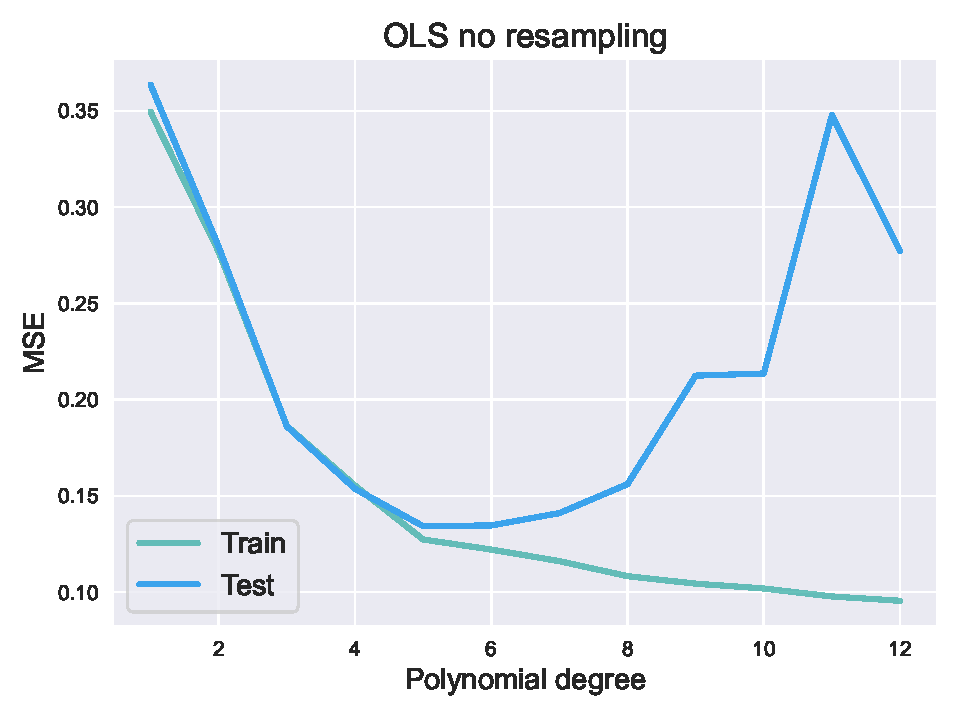
\includegraphics[width=\linewidth]{OLS_mse_noresample.pdf}
                    \caption{Showing the MSE score for OLS, calculated on the train and test sample for different polynomial degrees.}
                    \label{fig:res:OLS_mse_noresample}
                \end{figure}

                \begin{figure}[H]
                    \centering
                    \includegraphics[width=\linewidth]{OLS_r2_noresample.pdf}
                    \caption{Showing the $\Rsquared$ score for OLS, calculated on the train and test sample for different polynomial degrees.}
                    \label{fig:res:OLS_R2_noresample}
                \end{figure}

                To investigate the stability of our fits with varying polynomial degrees, we also plot coefficient values with varying polynomial degree. In Figure~\ref{fig:res:OLS_beta_values_plot} we see these plotted for $p = 1,2,3$ with 95\% confidence intervals. These are calculated using the diagonal $\sigma^2_{\theta_a} = \var{(\vec{\hat{\theta}})_{aa}}$. Additionally, in Figure~\ref{fig:res:OLS_beta_values_table} we see the values of these coefficients tabulated for $p \in [1,5]$.

            \begin{figure*}
                \begin{subfigure}{\textwidth}
                    \centering
                    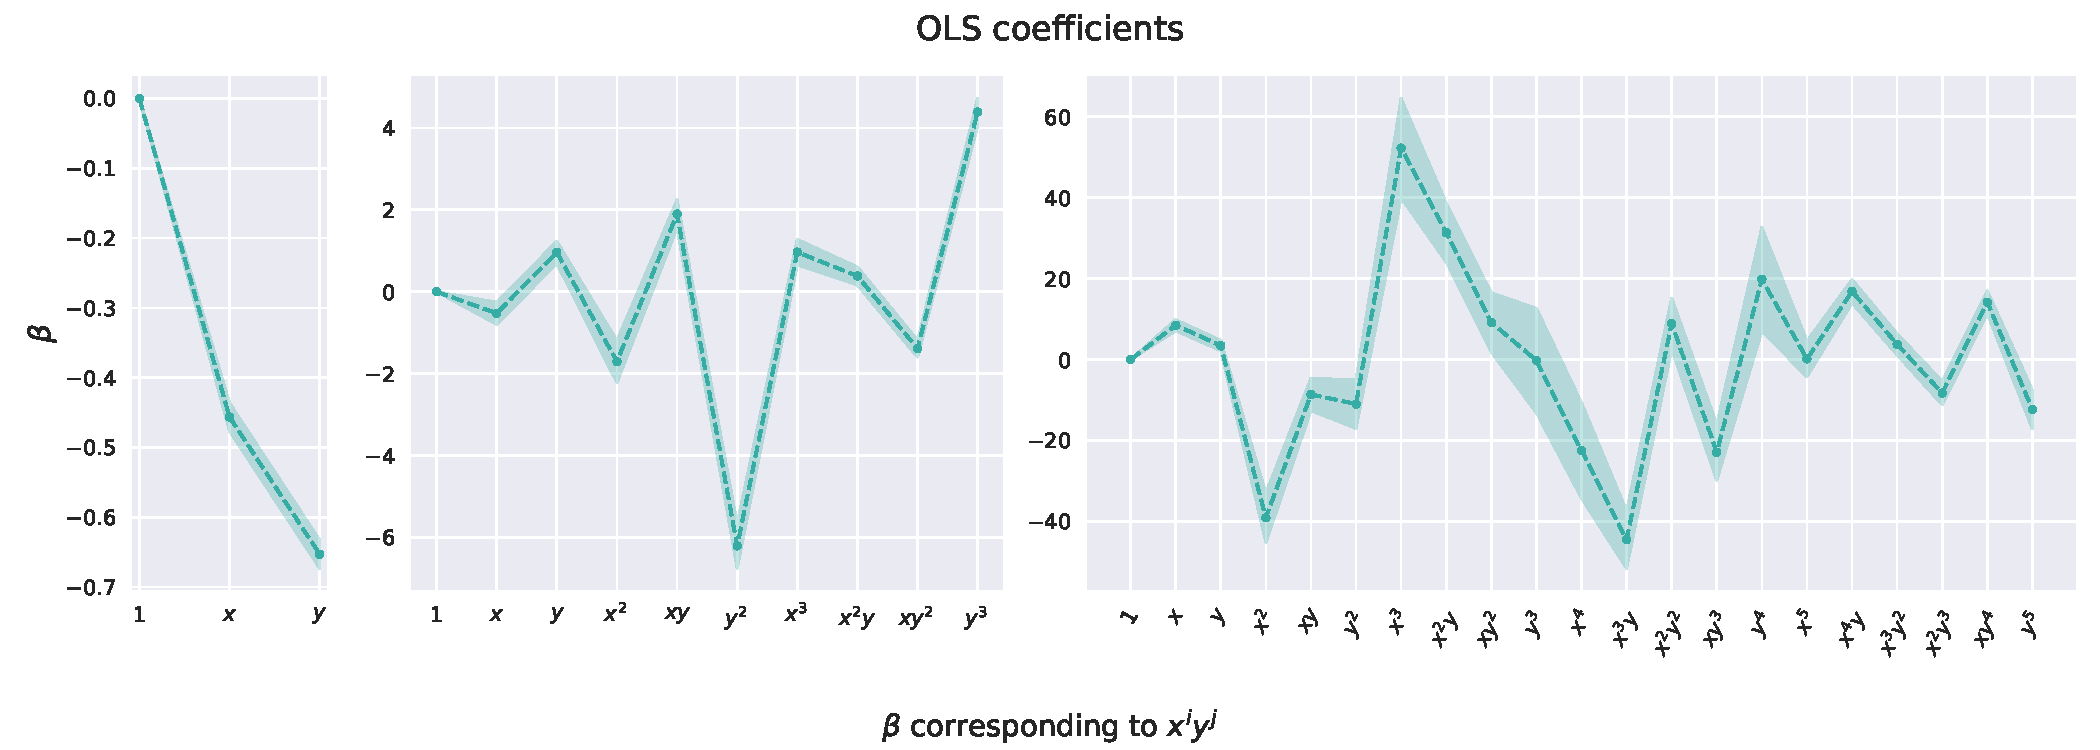
\includegraphics[width=\linewidth]{OLS_coefs_plots.pdf}
                    \caption{Showing values of polynomial coefficients for degree 1, 3 and 5 from left to right. The shaded regions are given by $\pm 2\sigma_\theta$. Note the different y-axes.} 
                    \label{fig:res:OLS_beta_values_plot}
                \end{subfigure}
                \begin{subfigure}{\textwidth}
                    \centering
                    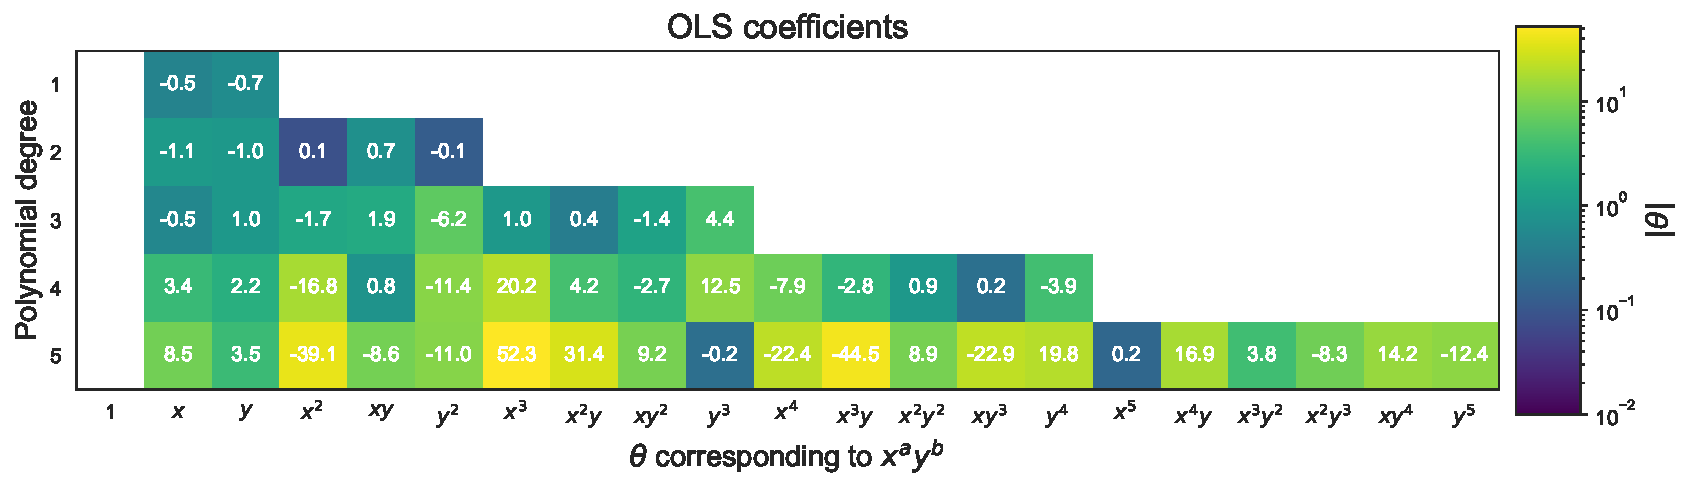
\includegraphics[width=\linewidth]{OLS_coefs_table.pdf}
                    \caption{Showing $\theta_{ab}$ corresponding to the term $x^a y^b$ present in the fit.}
                    \label{fig:res:OLS_beta_values_table}    
                \end{subfigure}
            \end{figure*} 


            The metrics thus far have been calculated without the use of any resampling techniques. To see how this influences MSE, we apply $k$-fold Cross-validation and plot the averaged train- and test MSE across the different folds. This is presented in Figure~\ref{fig:res:OLS_mse_kfold}. The optimal polynomial degrees and MSE values based on the training data is presented in Table~\ref{res:tab:OLS_kfold_optimal}



            \begin{table}[H]
                \centering
                \begin{tabular}{l|ll}
                $k$ & $\msub{p}{opt}$ & MSE \\
                \hline
                5   & 6         & 0.136 \\
                7   & 7         & 0.134 \\
                10  & 7         & 0.136
                \end{tabular}
                \caption{Showing the optimal degrees $\msub{p}{opt}$ and MSE values calculate on the test data using cross validation with $k = 5, 7$ and $10$.}
                \label{res:tab:OLS_kfold_optimal}
            \end{table}
            
            Just as in the case without resampling, the train MSE decreases with $p$. For the test MSE, the increase after the various $\msub{p}{opt}$ values is smaller, but the general trend is the same. For further usage of Cross-validation as a resampling technique applied to the Franke data, we use $k = 7$.   
            
            \begin{figure}[H]
                \centering
                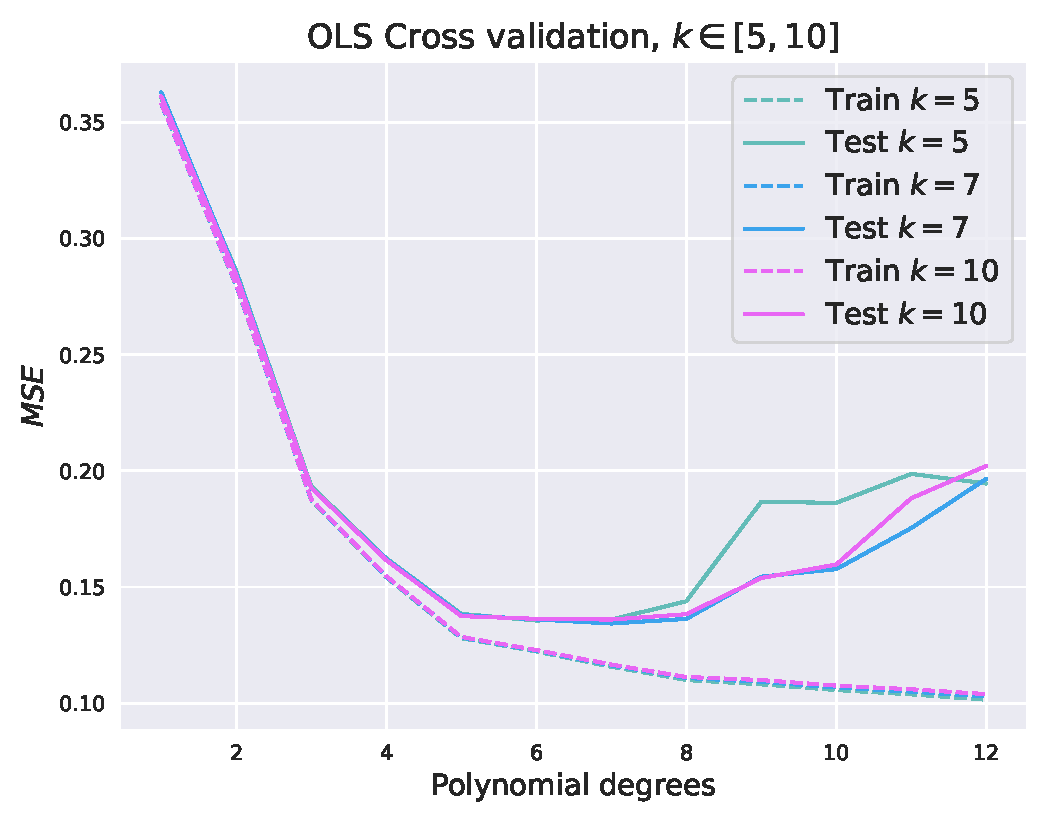
\includegraphics[width=\linewidth]{OLS_mse_kfold.pdf}
                \caption{MSE values as a function of polynomial degrees, calculated using $k$-fold Cross validation for $k = 5, 7$ and $10$. }
                \label{fig:res:OLS_mse_kfold}
            \end{figure}

            \comment{Reminder: Compare bootstrap and CV.}

        
        \subsubsection*{Exploring Resampling}
            There are some parameters that need to be set before resampling.
            \comment{Reminder: Insert bootstrap results.}
            \begin{figure}[ht]
                \centering
                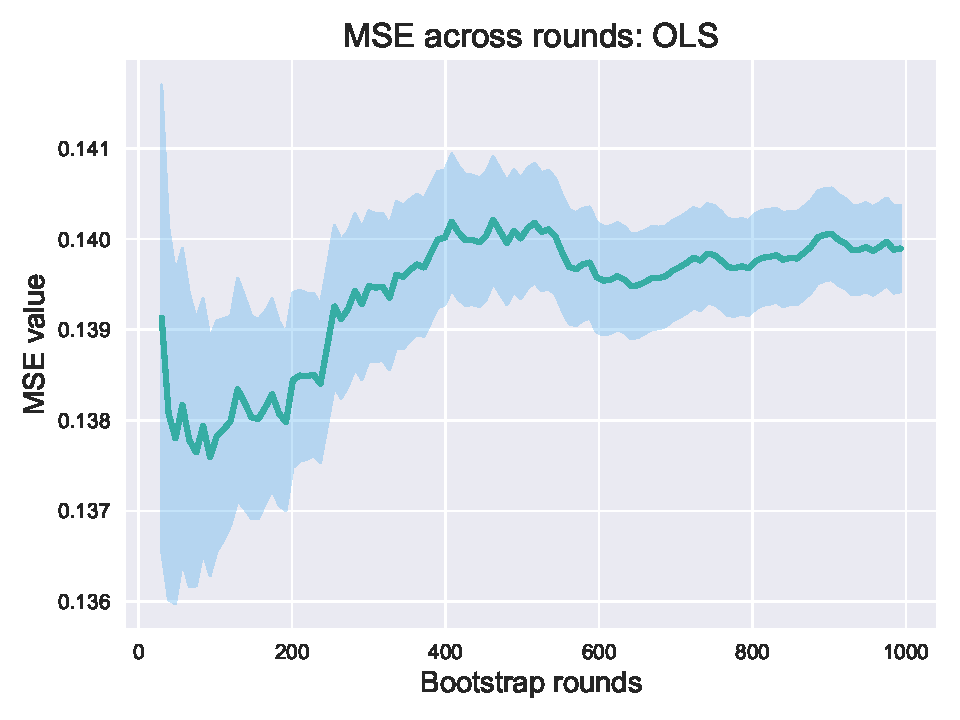
\includegraphics[width=\linewidth]{BS_mse_across_rounds_OLS.pdf}
                \caption{Plot of the MSE value as a function of number of bootstrap rounds.}
                \label{res:fig:mse across rounds}
            \end{figure}

            \begin{figure}[ht]
                \centering
                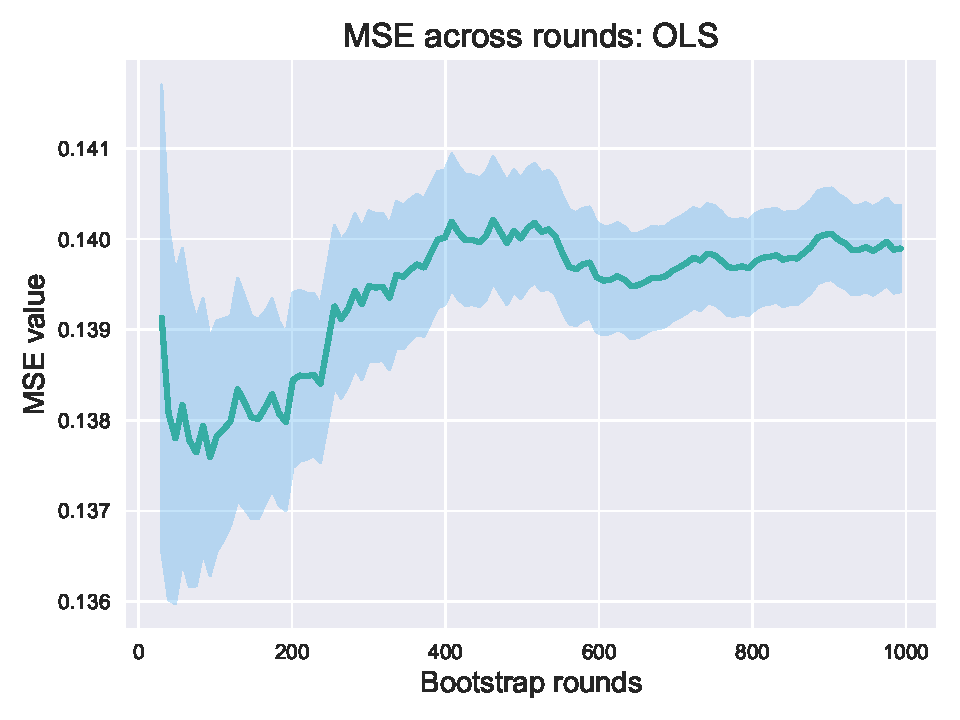
\includegraphics[width=\linewidth]{BS_mse_across_rounds_OLS.pdf}
                \caption{}
                \label{}
            \end{figure}


        \subsubsection*{Applying Resampling}
            \begin{figure}[H]
                \centering
                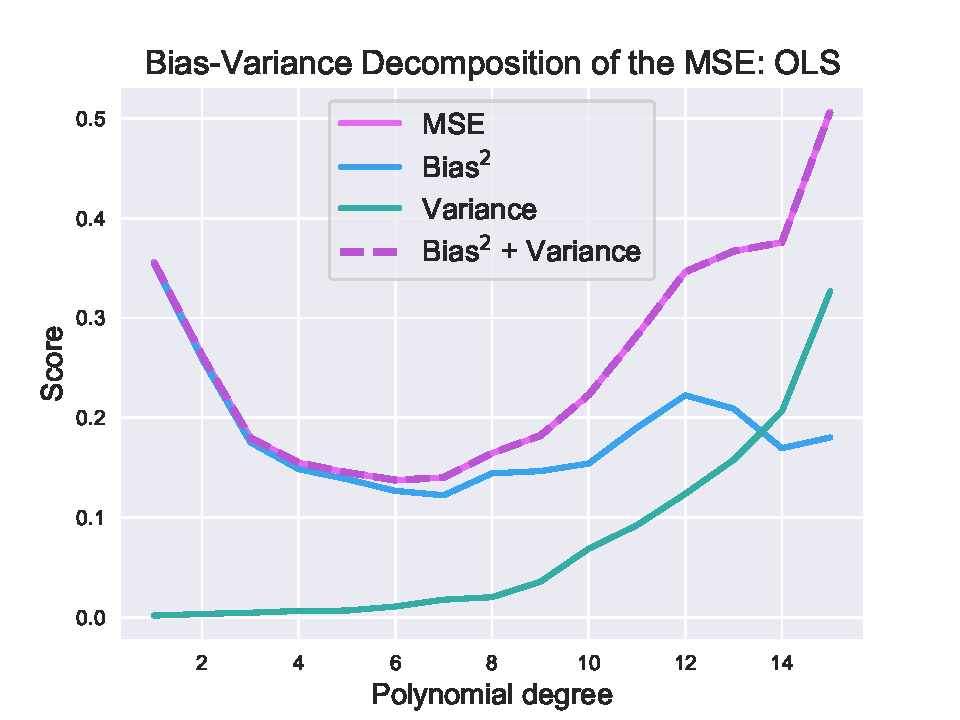
\includegraphics[width=\linewidth]{BS_Bias_var_decomp_OLS.pdf}
                \caption{FILL ME}
                \label{fig:res:OLS_bias_variance_tradeoff}
            \end{figure}
    

    \subsection{Ridge and Lasso}
        \comment{No naïveté, exploration of resampling is just 1 sentence.}\\
        We now repeat the same analysis for ridge and Lasso regression. \comment{Add plots for task C repeated for Ridge and Lasso (parts of task e and f)}
        
        We preform the save Cross-validation analysis as we did for OLS. This has been done for two different $\lambda$ values, $0.1$ and $10^{-7}$. This can be seen in Figures~\ref{res:fig:ridge_cv_badlambda} and~\ref{res:fig:ridge_cv_goodlambda} respectively.
        \begin{figure}[ht]
            \begin{subfigure}{\linewidth}
                \centering
                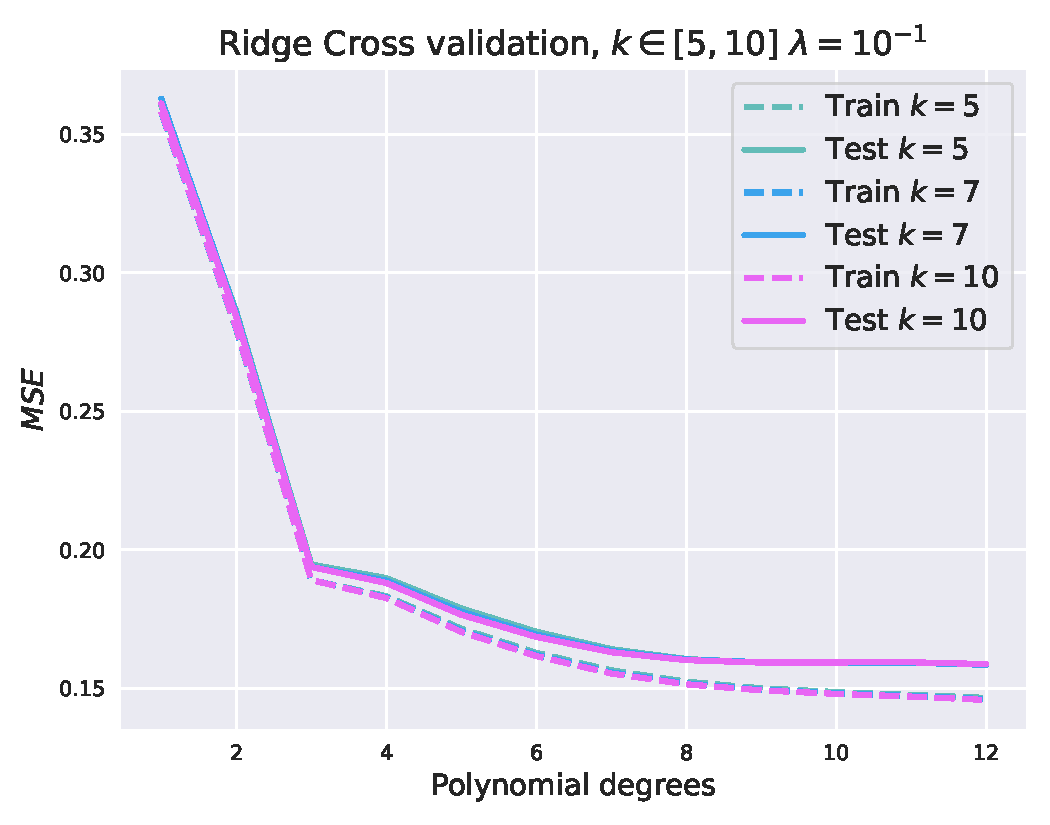
\includegraphics[width=\linewidth]{bad_lmbda_Ridge_mse_kfold.pdf}
            \end{subfigure}
            \caption{Test and train MSE calculated across different polynomial degrees using Ridge regression for $\lambda = 10^{-1}$}
            \label{res:fig:ridge_cv_badlambda}
            \begin{subfigure}{\linewidth}
                \centering
                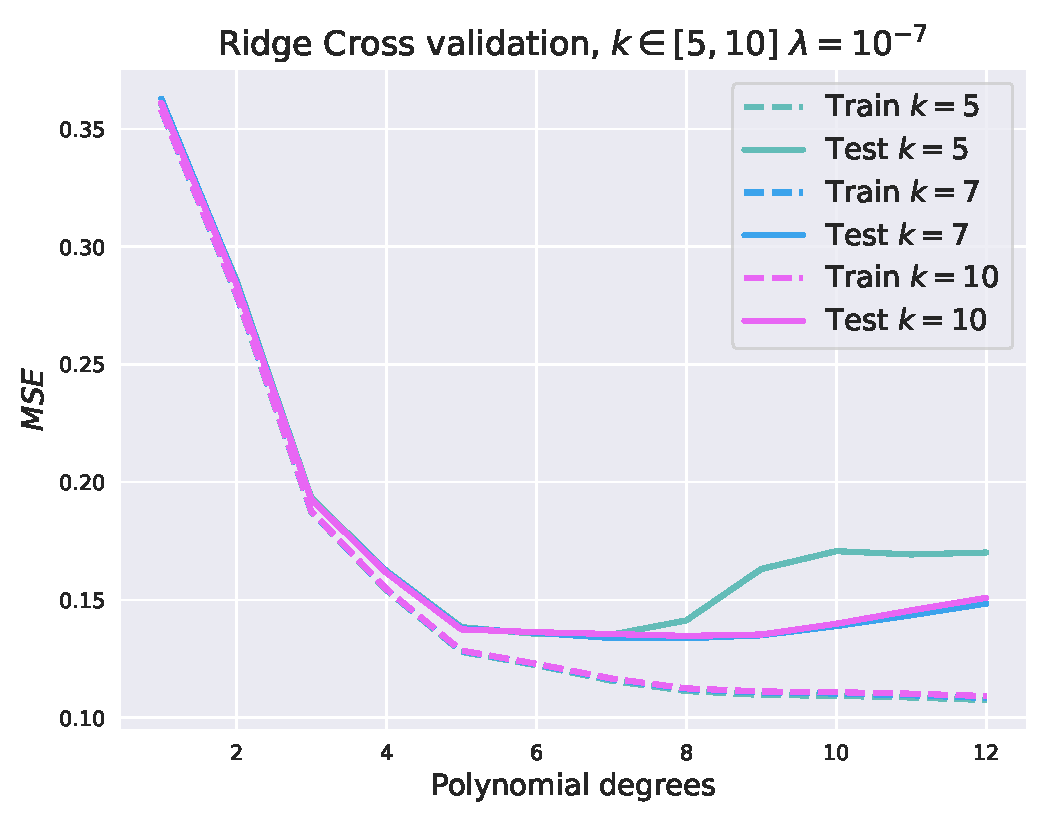
\includegraphics[width=\linewidth]{good_lmbda_Ridge_mse_kfold.pdf}
            \end{subfigure}
            \caption{Test and train MSE calculated across different polynomial degrees using Ridge regression for $\lambda = 10^{-7}$}
            \label{res:fig:ridge_cv_goodlambda}
        \end{figure}

        Moving on to Lasso regression, we try the same $\lambda$ values of $0.1$ and $10^{-7}$. 

        \begin{figure}[ht]
            \begin{subfigure}{\linewidth}
                \centering
                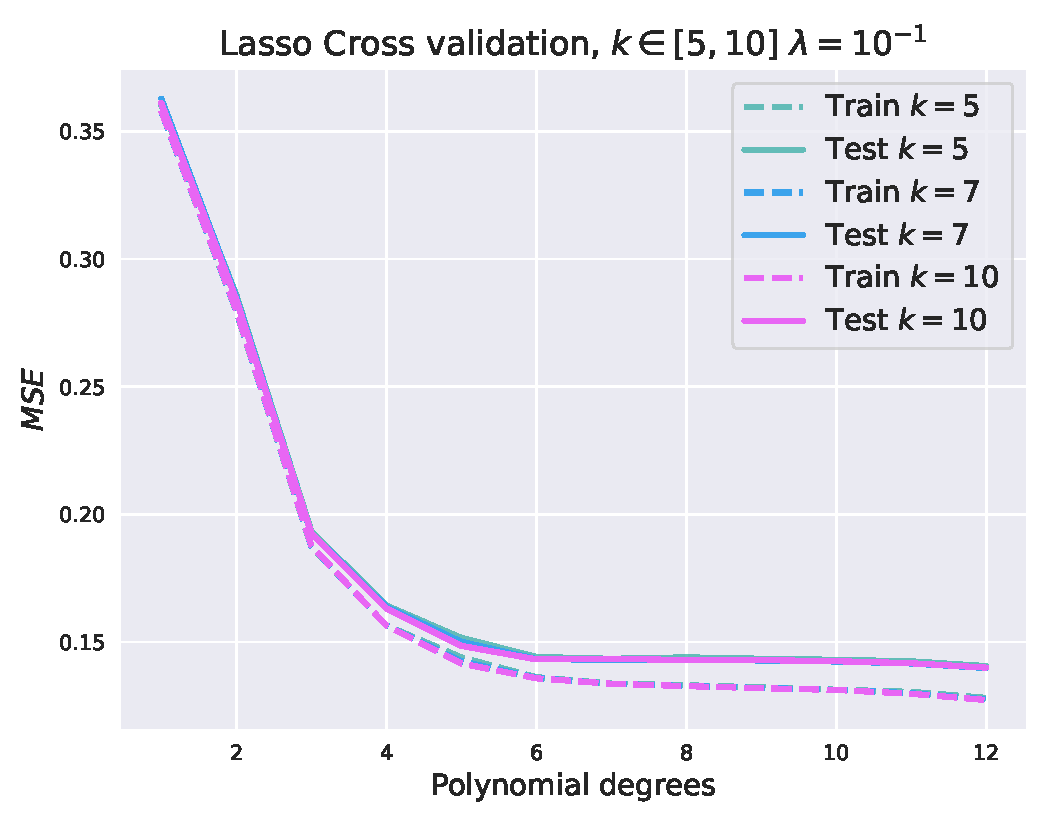
\includegraphics[width=\linewidth]{bad_lmbda_Lasso_mse_kfold.pdf}
            \end{subfigure}
            \caption{Test and train MSE calculated across different polynomial degrees using Lasso regression for $\lambda = 10^{-1}$}
            \label{res:fig:lasso_cv_badlambda}
            \begin{subfigure}{\linewidth}
                \centering
                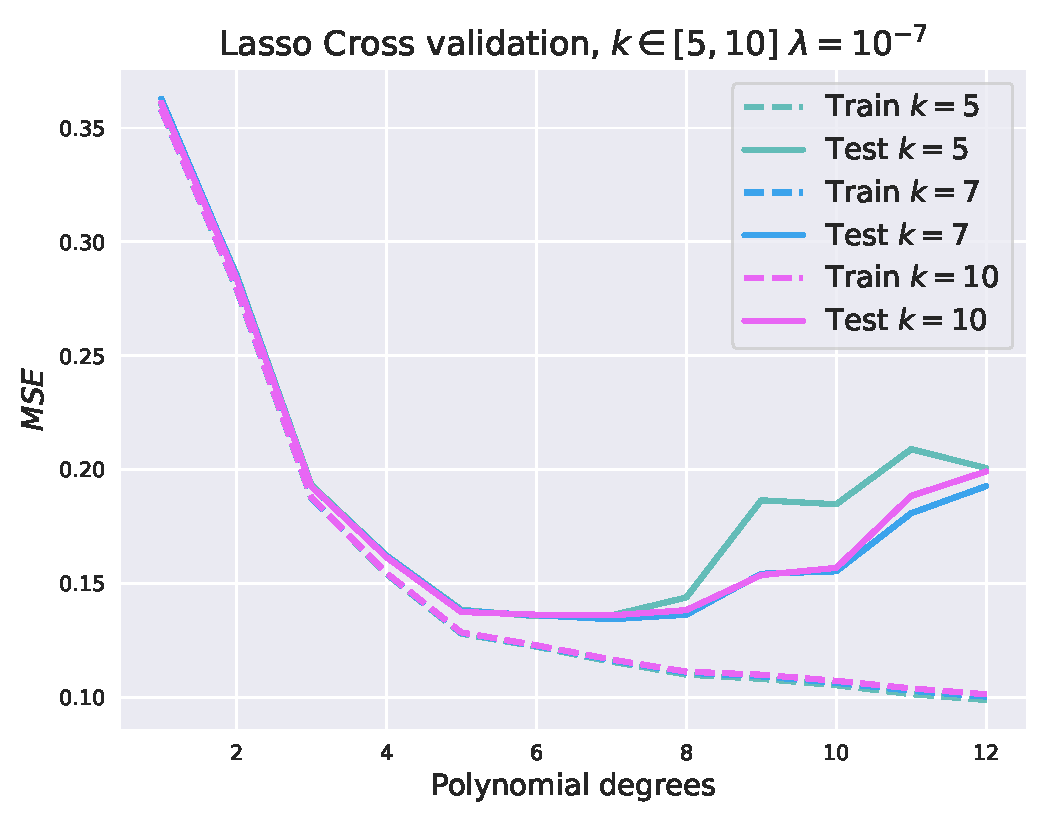
\includegraphics[width=\linewidth]{good_lmbda_Lasso_mse_kfold.pdf}
            \end{subfigure}
            \caption{Test and train MSE calculated across different polynomial degrees using Lasso regression for $\lambda = 10^{-7}$}
            \label{res:fig:lasso_cv_goodlambda}
        \end{figure}

        \begin{figure}[ht]
            \begin{subfigure}{\linewidth}
                \centering
                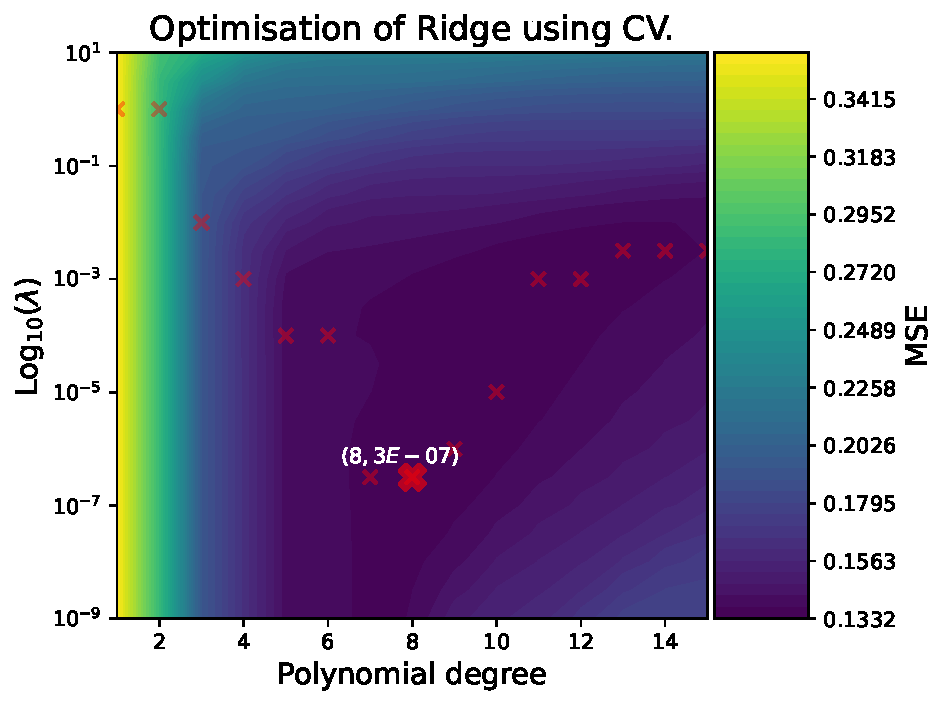
\includegraphics[width=\linewidth]{heatmap_ridge.pdf}
            \end{subfigure}
            \begin{subfigure}{\linewidth}
                \centering
                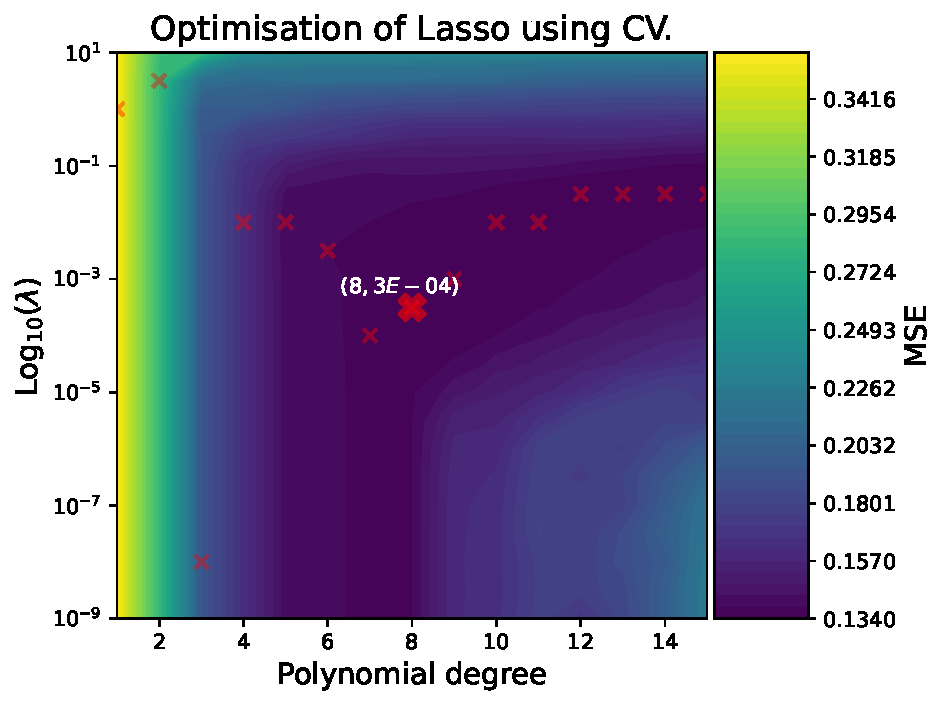
\includegraphics[width=\linewidth]{heatmap_lasso.pdf}
            \end{subfigure}
            \caption{Grid search of the MSE of the ridge and Lasso methods fitted to the Franke function with $k=7$ CV resampling. The red crosses denote the best $\lambda$-value for each degree, the large cross denoting the global minimum of the MSE.}
            \label{fig:res:Franke_heatmaps}
        \end{figure}


    \subsection{Nicaraguan terrain data}
        
        \begin{figure} [ht]
            \centering
            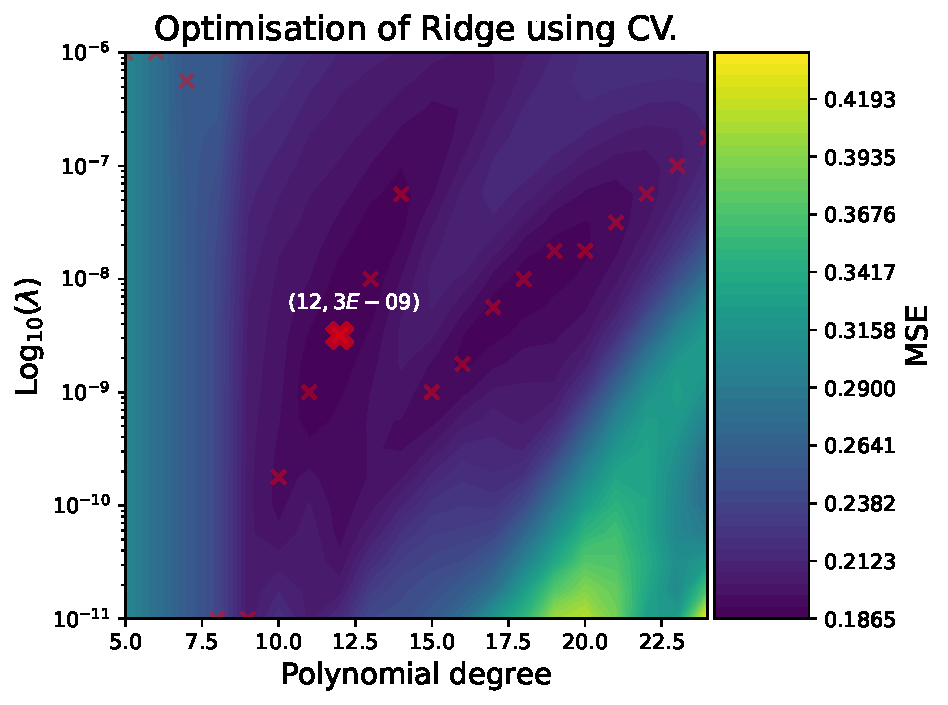
\includegraphics[width=\linewidth]{HM_Nica_Ridge_heatmap.pdf}
            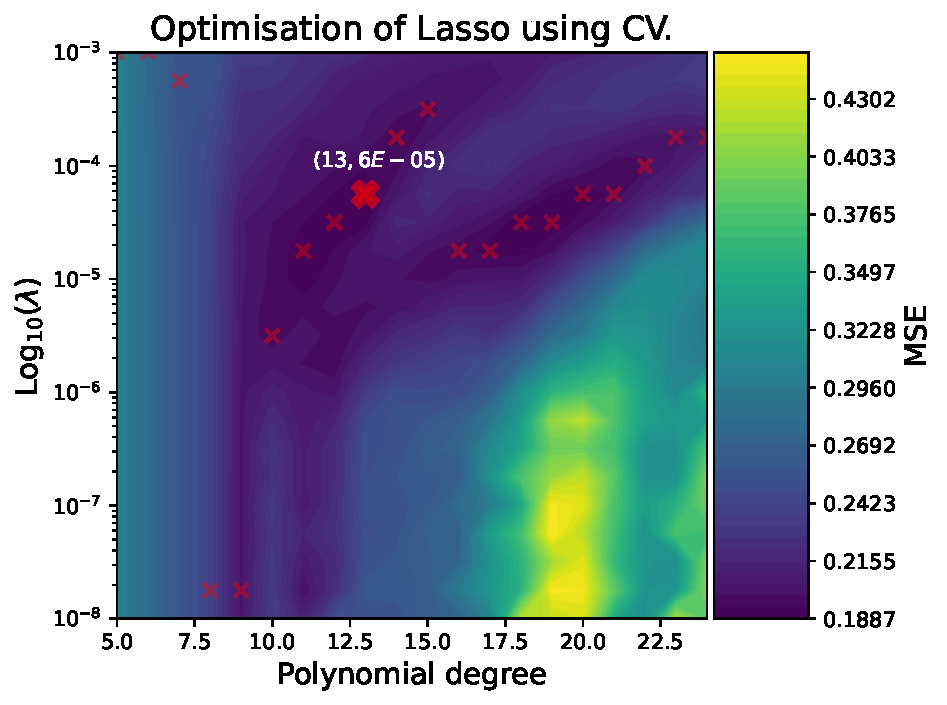
\includegraphics[width=\linewidth]{HM_Nica_Lasso_heatmap.pdf}
            \caption{Grid search of the MSE of the ridge and Lasso methods fitted to Nicaraguan terrain data with $k=7$ CV resampling. The red crosses denote the best $\lambda$-value for each degree, the large cross denoting the global minimum of the MSE.}
            \label{res:fig:Nica_heatmap}
        \end{figure}
    
\section{Discussion}
    \subsection{Data scaling}
        \comment{This should probably be a subsubsection within something else. Just summing up the thoughts we have thrown around regarding the necessity and function of scaling.}
        \comment{Please read and see if it makes sense at all!}
        The scaling of the inputs and measurments can roughly be divided into two operations, each with their own set consequences. Let us first consider shifting of the measurements $\vec{y}$ and the inputs $\vec{x}_a$ by their respective means. Effectively, this eliminates a degree of freedom from our model $\hat{f}(x)$ as we set its mean value to zero, and leave out any parameter that would govern the intercept $\hat{f}(0)$. However, if we shift $\vec{y}$ to have zero mean as well, this degree of freedom becomes redundant, and we end up effectively reducing the dimensionality of the model by one. Moreover, in regularised models where some norm of the parameters $\norm[p]{\vec{\theta}}$ is penalised, we remove any penalisation of the choice of the intercept. This is natural to do, as the goal of these methods is to reduce the variance of the model, something which is not affected by changing the intercept.

        Considering now the rescaling of $\vec{y}$ and $\vec{x}_a$, these affect the fitting of the model more subtely. Looking at it through the lense of dimensionality know that
        \begin{align}
            \dimof{\theta_a} = \dimof{y} / \dimof{x_a}.
        \end{align}
        From this we can infer that the order of magnitude of a parameter $\theta_a$ is governed by the dimension its corresponding feature $\dimof{x_a}$. This matters in the regularised models where a cost is associated with the norm of the parameters $\norm[p]{\vec{\theta}}$, which will be dominated by parameters whose dimension is large. In practice, this means that the fitting will focus more on reducing the magnitude of the parameters whose associated dimension is large, letting the others fluctuate more freely. By making the $x_a$'s dimensionless, the parameters are put on a `level playing field', so to speak. The dimension of $y$ serves to raise or lower the order of magnitude of the all the parameters equally, and can be adjusted as to avoid numerical truncation errors by avoiding larger floats.

        From this, we can conclude that scaling of the inputs is not strictly necessary when using OLS, as there is no regularisation penalty associated with the dimension of the parameters. However, the MSE is still a dimensionful quantity, and it is useful then to scale the data for OLS too for consistency and ease of comparison of the results between the models.

    \subsection{OLS}
        Looking back at Figures~\ref{fig:res:OLS_mse_noresample} and~\ref{fig:res:OLS_R2_noresample} showing the MSE and $\Rsquared$ scores calculated using the train and test set, we recognise a common sign of overfitting when moving past $\msub{p}{opt} = 5$. Since the polynomial degree increases, we can make many more $x^ay^b$ combination, which in turn gives more coefficients $\theta_{ab}$ to determine. This introduces many new degrees of freedom to the fit, which allows our model to accurately recreate the exact points present in the training set, but at the cost of fitting the added noise $\epsilon$ and/or assuming a too complex structure to the underlying function $f(x)$. This can be seen by the large MSE values calculated on the test data, telling us that our model preforms poorly on data which it has not yet been exposed to.

    \subsection{Resampling}
        \comment{Here I am just writing a bit on our discussion about the limit of resampling. Structure of the discussion section is very much not set in any stone.}
        Resampling a given data set seems on the face of it to be truly the work of magic. Somehow we invoke the law of large samples from the central limit theorem~\eqref{theo:eq:CLM} that our statistical quantities, like the mean value, approaches the true value as the sample size grows. However, that is not exactly what we are doing when we are resampling. To illustrate this, we can think of a coin-flipping experiment where are results are categorically heads or tails. If we perform the experiment an \textit{odd} number of times, we must necessarily end up with either more heads or more tails. If we then continously resample from this dataset, a mean value should by the central limit theorem rather approach the \textit{biased} mean value of the original dataset.

        The value of resampling rather comes from creating a way to emphasise different parts of the original dataset when fitting our model, and consequently comparing what this does to the predictions of the model. For instance, an overfitted model might contort to accomodate a statistical outlier in the original dataset, and thereby make a poor prediction on new data. However, when resampling, many of the new datasets sampled to make new fits from our model will not include this statistical outlier, and should make predictions not influenced too heavily by this. There should then be a medium where the particular `oddities' in the original dataset can be smoothed over, and the bias of the original dataset is not brought out to the front.

        \subsubsection*{Cross validation and bootstrap} 
            The choice of $k=7$ used for our parameter grid search is influenced by the computational aspect of the approach. Since a model has to be fitted $k$ times for each set of parameter $(p,\lambda)$, it is clear that this increases the time taken to search the parameter space. However, for both OLS and Ridge, the closed form expressions (Eqs.~\eqref{theo:eq:OLS_coefs} and~\eqref{theo:eq:Ridge_coefs} respectively) only require matrix multiplication and inversion. Adding more folds chould (\comment{nice one}) potentially be feasible here. However, since Lasso requires a cost function minimization, it is significantly slower than OLS and Ridge, espcially for high $p$. Therefor we get a trade-off between the number of $(p,\lambda)$ to try and the number of folds $k$, where $k=7$ was found to allow for high parameter resolution while still being completed in a feasible amount of time.
            \newline
            \comment{Some general disc about Bootstrapping here, and after that some comparison?}
            \newline
            The Bootstrap holds the test set constant during calculation of metrics. This is in contrast to Cross-validation where the test set is different (with no overlapping points) for each fitted model. Holding the test set constant might be beneficial since every model calculates metrics based on the same data, thus averaging over MSE scores gives a more accurate picture of the MSE present in that specific test set. However, this introduces bias since we assume that the selected test set accurately represents the population, which it may not. Cross-validation on the other hand does not average MSE values over the same test data and larger variations may occur. The advantage of this is that metrics are calculated on the entire data set, not just a specific partition.          

\section{Concluding remarks}

% for numbering appendix equations more appropriately
\numberwithin{equation}{section}
\renewcommand{\theequation}{\thesection.\arabic{equation}}
\begin{appendices}
    \section{Bias-variance decomposition of the MSE of a linear model} \label{app:sec:bvdecomp}
        The true MSE of a model $\hat{f}(x)$ to data constructed from $f(x) + \epsilon$ can be decomposed into terms resulting from the bias of the model, the variance of the model and the \textit{irreducible error} resulting from the error in the observations. The bias encapsulates tendency of the model $\hat{f}(x)$ to under- or overpredict the value at a point $x$ as the data used to fit the model is varied. The variance encapsulates how much the prediction at a point $x$ changes as the data used to fit the model is varied. The decomposition follows from the definition of the MSE. We supress the arguments $x$, understanding that the expectation values are taken at the same point $x$.

        \begin{align} \nonumber
            &\operatorname{MSE}(\hat{f}) = \expval\bclosed{(f+\epsilon-\hat{f})^2} \\ \nonumber
            =& \expval\bclosed{\pclosed{(f+\epsilon-\expval(\hat{f}))- (\hat{f}-\expval(\hat{f}))}^2} \\ \nonumber
            =& \expval\bclosed{\pclosed{f+\epsilon-\expval(\hat{f})}^2} + \expval\bclosed{\pclosed{\hat{f}-\expval(\hat{f})}^2} \\ \nonumber
            &-2 \expval\bclosed{ (f+\epsilon-\expval(\hat{f})) (\hat{f}-\expval(\hat{f})) } \\ \nonumber
            =& \pclosed{\expval\bclosed{f+\epsilon-\expval(\hat{f})}}^2 + \expval(\epsilon^2) + \var(\hat{f}) - 2\expval(\epsilon \hat{f}) \\
            =& \pclosed{\bias(\hat{f})}^2 + \var(\hat{f}) + \sigma^2,
        \end{align}
        where in the last line, we used that $\expval(\epsilon\hat{f}) = \expval(\epsilon)\expval(\hat{f})=0$.\footnote{At first glance, this might seem odd, as there is noise involved in the fitting of $\hat{f}$ too. However, under the assumption that the noise is i.i.d. between experiments, the noise in the data used to fit $\hat{f}$ is independent of the noise in a test sample. It is worth noting that this would not be true if we were comparing with the same data used to fit the model, which explains the optimism of the training MSE. \comment{This last part here might be put into the discussion perhaps?}}

    \section{Theoretical proof of concept of the OLS model} \label{app:sec:OLS_proof}
        Supposing that we have have data generated from from $y_i = f(x_i)+\epsilon$ as before, we look statistical quantities derived from the distribution of our parameters $\vec{\theta}$ inhereted from $\epsilon\distas \normal{0}{\sigma^2}$. Under the assumption that $f(x) \in \operatorname{span}\cclosed{x}_a, a\in 1,\ldots,p$ of our design matrix $X$, we can write the data $\vec{y} = X\vec{\theta} + \vec{\epsilon}$ for some $\vec{\theta}$ which would be a `true' optimum for our parameters.

        The expectation value of a datapoint $y_i$ is\footnote{In this appendix, we understand repeated indices to be summed over.}
        \begin{align}
            \expval(y_i) = \expval\bclosed{X_{ia} \theta_a + \epsilon_i} = X_{ia}\theta_a + \expval(\epsilon_i) = X_{ia}\theta_a,
        \end{align}
        with its variance is
        \begin{align} \nonumber
            \var(y_i) &= \expval\bclosed{\pclosed{y_i-\expval\pclosed{y_i}}^2} = \expval\bclosed{\pclosed{X_{ia}\theta_a + \epsilon_i - X_{ia}\theta_a}^2} \\
            &= \expval\pclosed{\epsilon_i^2} = \var\pclosed{\epsilon_i} = \sigma^2.
        \end{align}

        The expectation value of our parameters can be calculated specific to OLS as
        \begin{align} \nonumber
            \expval(\vec{\thetahat}) &= \expval\bclosed{(X^TX)^{-1}X^T \vec{y}} = \expval\bclosed{(X^TX)^{-1}X^T \bclosed{X\vec{\theta} + \vec{\epsilon}} } \\
            &= \expval\pclosed{\vec{\theta}} + {(X^TX)}^{-1}X^T \expval\pclosed{\vec{\epsilon}} = \vec{\theta},
        \end{align}
        and their covariance matrix is
        \begin{align} \nonumber
            \var(\vec{\thetahat}) &= \expval({\vec{\thetahat} \vec{\thetahat}^T}) - \expval({\vec{\thetahat}}) \expval({\vec{\thetahat}^T}) \\ \nonumber
            &= \expval\bclosed{(X^TX)^{-1}X^T \vec{y} \vec{y}^T X (X^TX)^{-1}} - \vec{\theta}\vec{\theta}^T \\ \nonumber
            &= (X^TX)^{-1}X^T \bclosed{X\vec{\theta}\vec{\theta}^TX^T + \sigma^2 \eye}X (X^TX)^{-1} - \vec{\theta}\vec{\theta}^T \\
            &= \sigma^2 (X^TX)^{-1},
        \end{align}
        where we have used that \(\expval(\vec{y}\vec{y}^T) = \expval\bclosed{(X\vec{\theta}+\vec{\epsilon})(X\vec{\theta}+\vec{\epsilon})^T} = X\vec{\theta}\vec{\theta}^TX^T + \sigma^2 \eye\).


    \section{Parameters for artifical data} \label{app:sec:frankefunction N and sigma}
        To fairly compare between methods, a constant number of sampled points $N$ from the Franke function (Eq.~\ref{met:eq:Franke_Function}) and the noise magnitude $\sigma$ needs to be set. We decided that $N = 600$ points should be sufficient to get enough data points in both the train and test set, while still being small enough to not bring in too much computational complexity. The points $(x,y)$ are drawn from a uniform distribution $x,y \distas \mathcal{U}(0,1)$ limited to their domain. Trough visual inspection, we decided on $\sigma = 0.1$ for the noise $\epsilon \distas \normal{0}{\sigma^2}$. We found that this scale gave our function plenty of noise, while still being recognizable (Figure~\ref{fig:app:frankefunction varying noise}).   
        \begin{figure*}
            \begin{subfigure}{.5\textwidth}
                \centering
                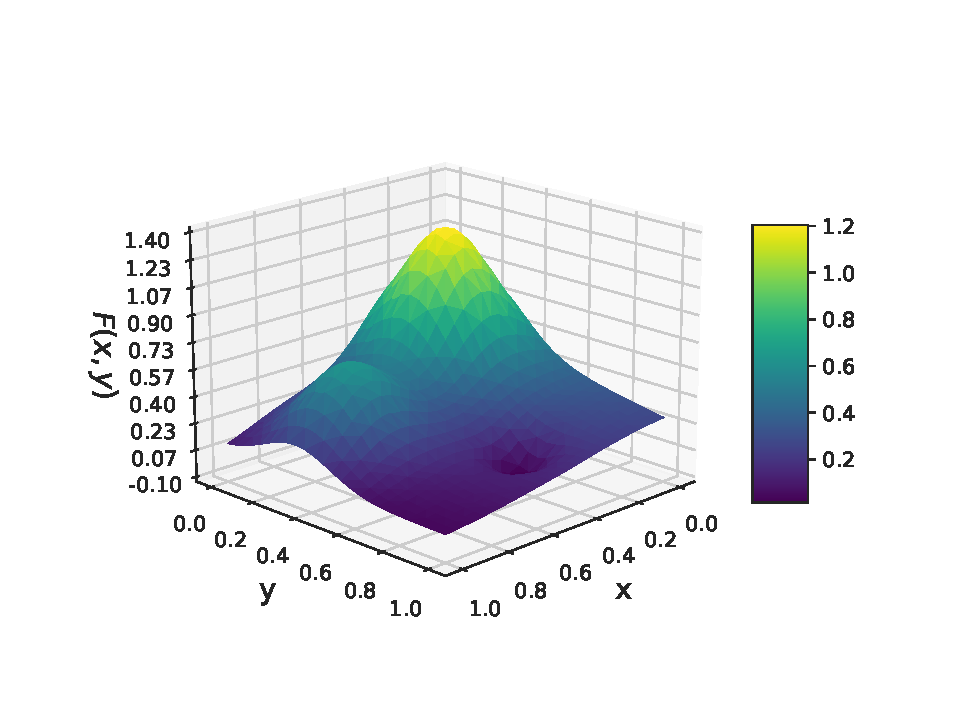
\includegraphics[width=\linewidth]{franke_functions_0.pdf}
                \caption{$\sigma = 0$}
                \end{subfigure}
            \hfill
            \begin{subfigure}{.5\textwidth}
                \centering
                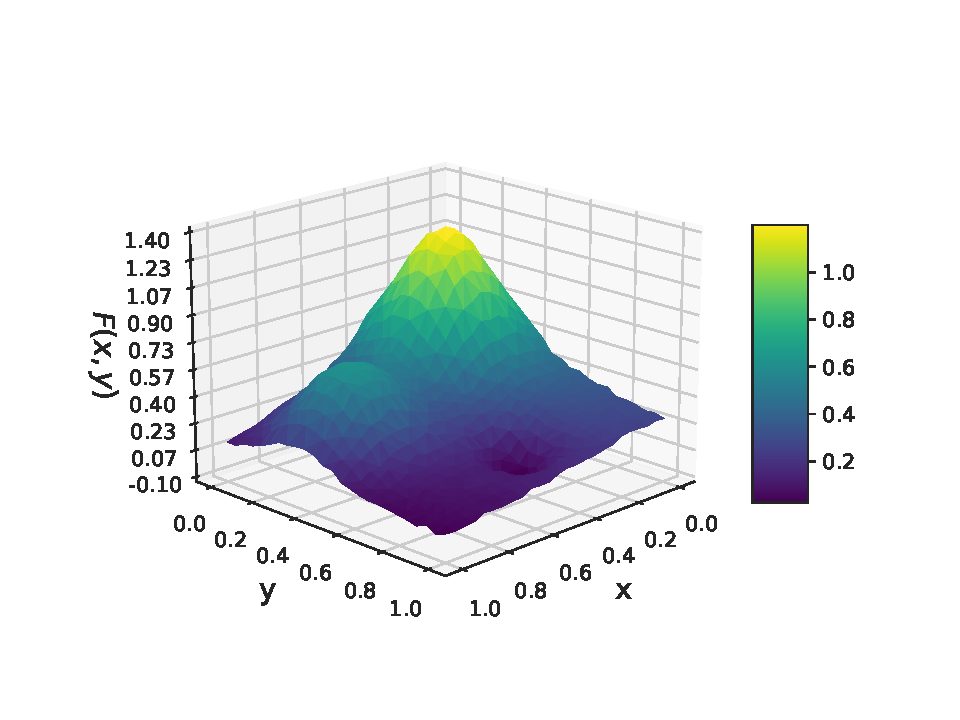
\includegraphics[width=\linewidth]{franke_functions_0_01.pdf}
                \caption{$\sigma = 0.01$}
            \end{subfigure}
            \hfill
            \begin{subfigure}{.5\textwidth}
                \centering
                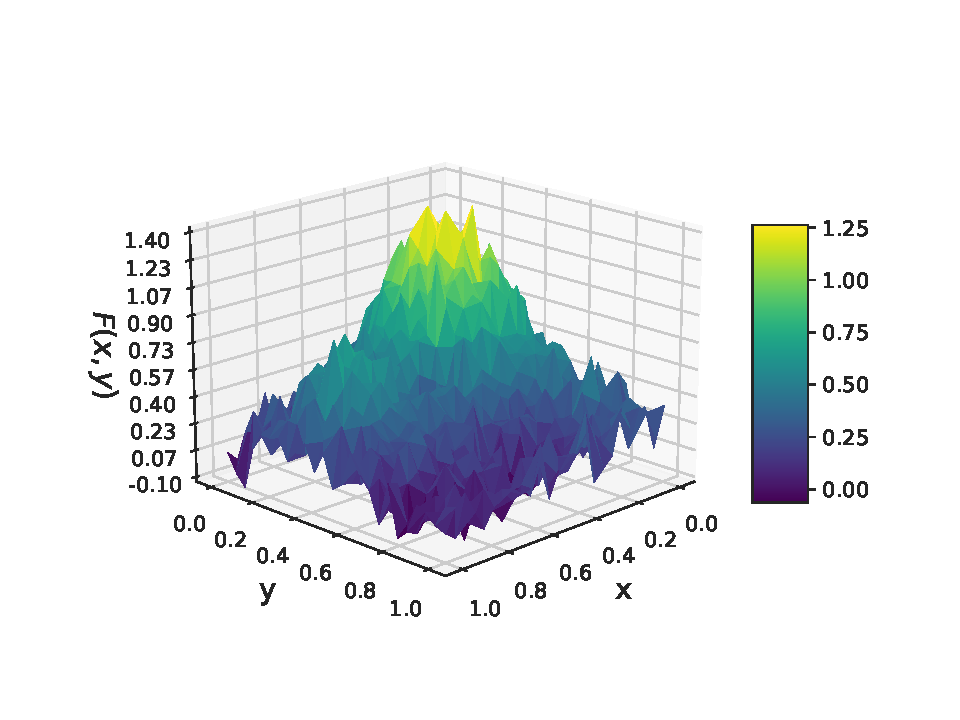
\includegraphics[width=\linewidth]{franke_functions_0_1.pdf}
                \caption{$\sigma = 0.1$}
            \end{subfigure}
            \begin{subfigure}{.5\textwidth}
                \centering
                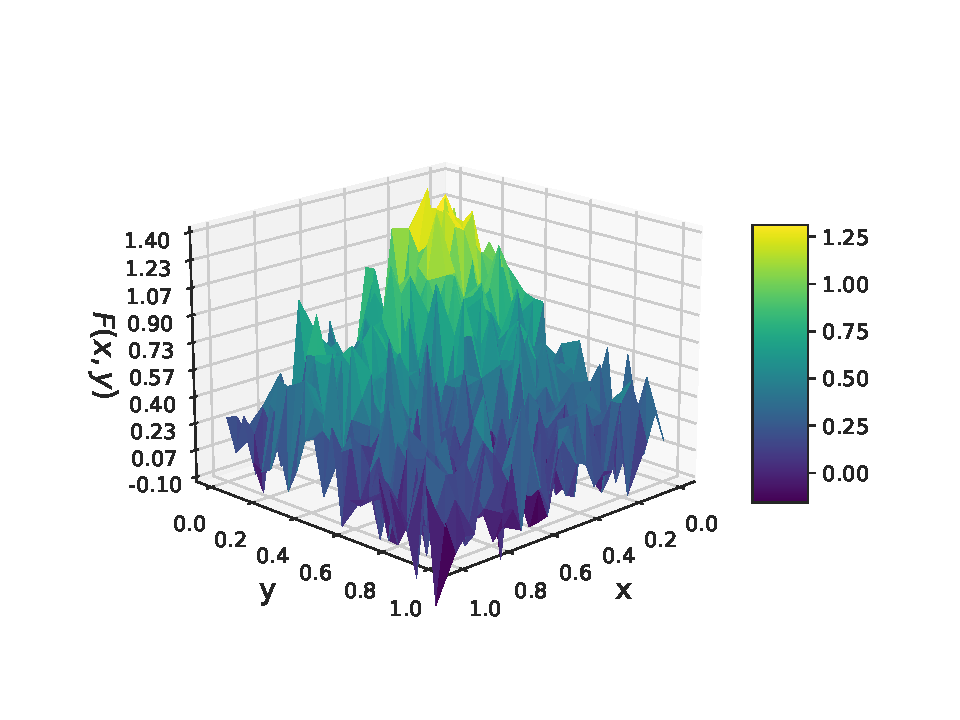
\includegraphics[width=\linewidth]{franke_functions_0_2.pdf}
                \caption{$\sigma = 0.2$}

            \end{subfigure}
        
            \caption{Showing Franke function with increasing noise, from \textit{a} to \textit{d}, $\sigma \in \{ 0, 0.01, 0.1, 0.2\}$. All figures plotted with $n = 625$ equidistant $(x,y)$ points.}\label{fig:app:frankefunction varying noise}
        \end{figure*}

    
    \section{Exploring number of Bootstrap rounds} \label{app:sec:BS rounds}
        \comment{Add reference -\Anna}
         Figure~\ref{app:fig:histograms for rounds} shows that the distribution of MSE values derived from models trained on bootstrapped data set approaches a normal distribution as the number of bootstrap rounds increases, as the Central Limit Theorem states. In accordance with other results, one can see from the plots that when exceeding 400 rounds the distribution stabilises (see also Figure~\ref{res:fig:mse across rounds} for this result). As in Figure~\ref{} the histograms show that the training data gives a smaller and more consistent MSE value than the testing data. This holds across number of bootstrap rounds.
        \begin{figure*}
            \begin{subfigure}{.5\textwidth}
                \centering
                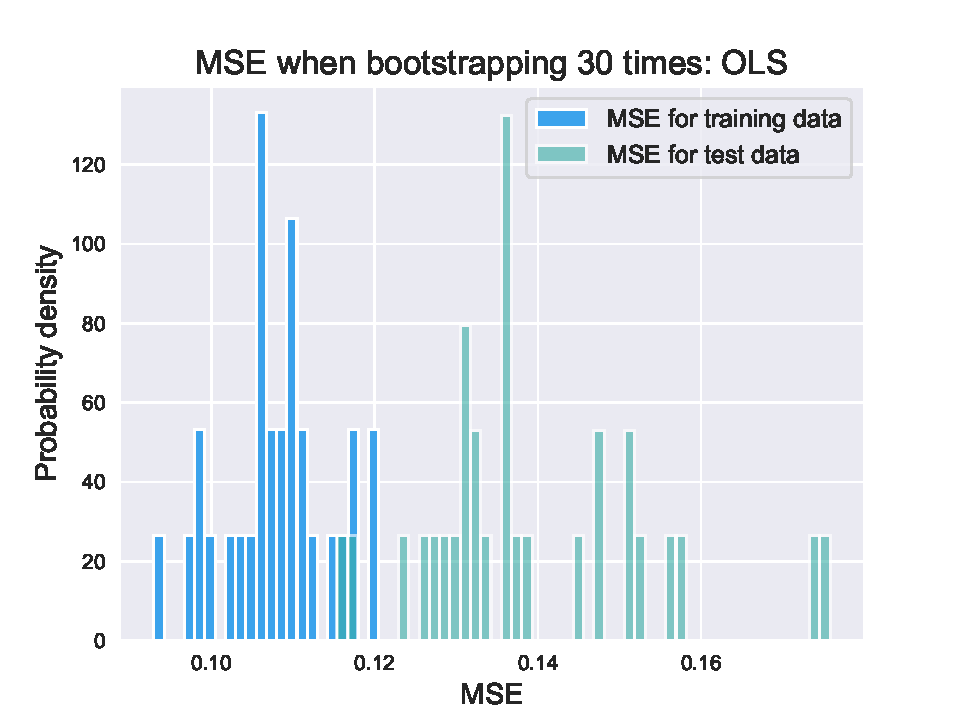
\includegraphics[width=\linewidth]{BS_hist_bootstraped_30_rounds_of_degree_7.pdf}
                \caption{}
                \label{app:fig:histograms for rounds:30}
                \end{subfigure}
            \hfill
            \begin{subfigure}{.5\textwidth}
                \centering
                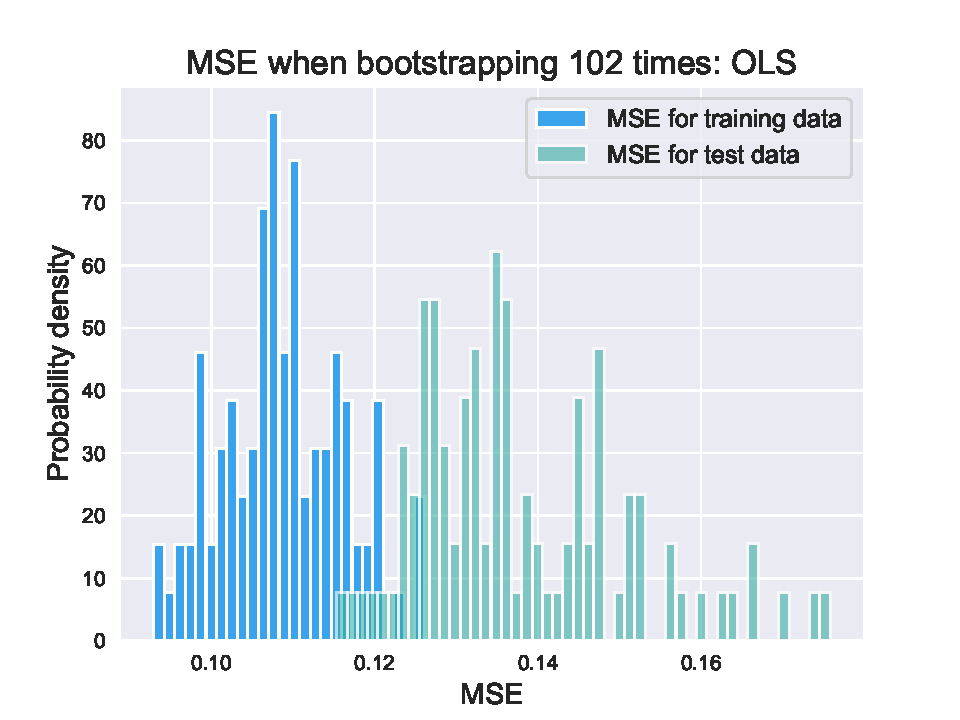
\includegraphics[width=\linewidth]{BS_hist_bootstraped_102_rounds_of_degree_7.pdf}
                \caption{}
                \label{app:fig:histograms for rounds:102}
            \end{subfigure}
            \hfill
            \begin{subfigure}{.5\textwidth}
                \centering
                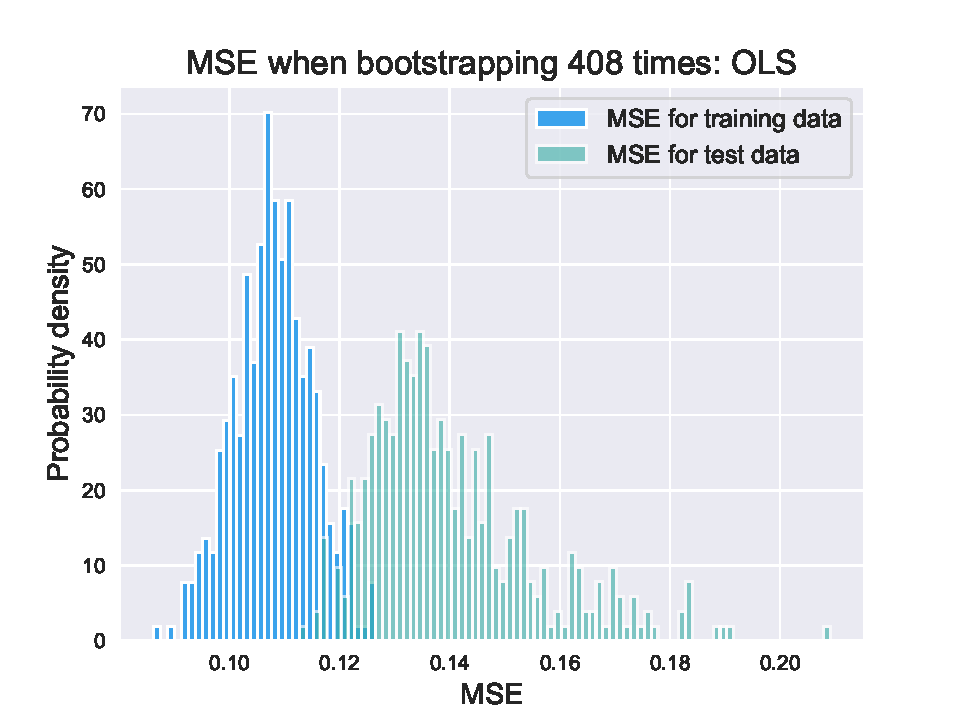
\includegraphics[width=\linewidth]{BS_hist_bootstraped_408_rounds_of_degree_7.pdf}
                \caption{}
                \label{app:fig:histograms for rounds:408}
            \end{subfigure}
            \begin{subfigure}{.5\textwidth}
                \centering
                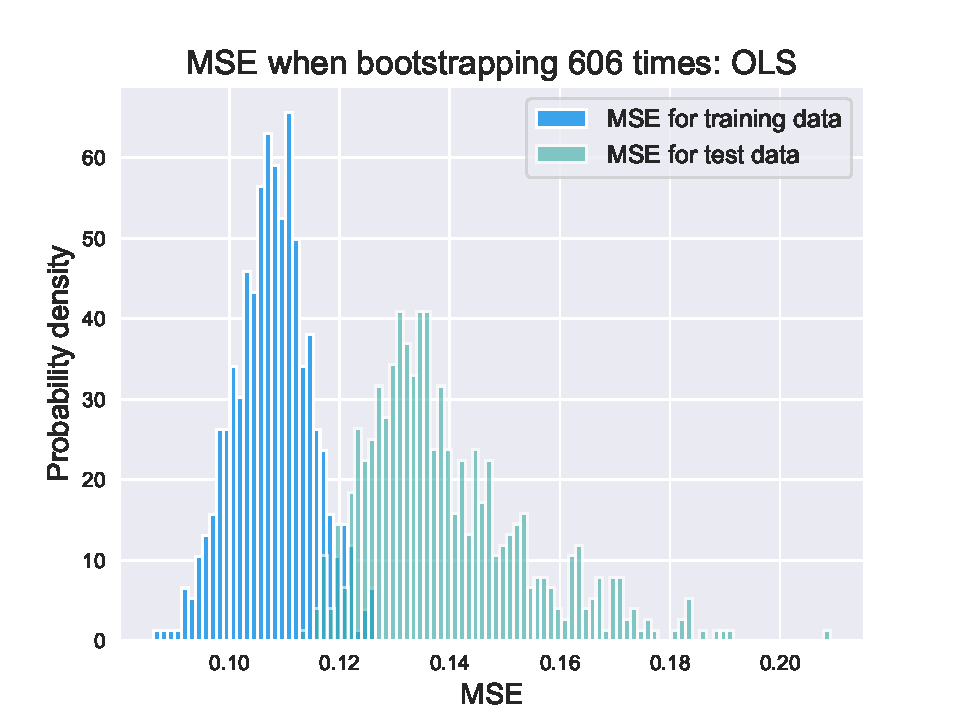
\includegraphics[width=\linewidth]{BS_hist_bootstraped_606_rounds_of_degree_7.pdf}
                \caption{}
                \label{app:fig:histograms for rounds:606}
            \end{subfigure}

            \caption{The histograms of MSE values for various number of bootstrap rounds. }
            \label{app:fig:histograms for rounds}
        \end{figure*}

\end{appendices}

\printbibliography

\end{document}

